\chapter{Ausgangsszenario}
\label{chapter:ausgangsszenario}

\section{Anforderungen}
\label{Anforderungen}

% kartografisches Produkt
Aktuelle Möglichkeiten der Datenerfassung über Sensoren und moderne Probenahmegeräte führen zu mehr und mehr Datensätzen, die für einen Landwirtschaftsbetrieb ausgewertet werden müssen. Darüber hinaus besteht die Notwendigkeit, Daten Jahresübergreifend und betriebsübergreifend auszuwerten, um pflanzenbauliche Zusammenhänge über statistische Methoden untersuchen zu können.
In den letzten 3 Jahren wurde beispielsweise nur zum Thema N-Versorgung\footnote{Stickstoffdüngung und -aufnahme} für einen Betrieb etwa 800 Datensätze mit 1,9 Mio Einträgen erfasst. Alle diese Daten haben einen räumlichen Bezug, sie müssen weiterverarbeitet, kartographisch aufbereitet und dargestellt werden.\\
Daraus ergeben sich verschiedenen Anforderungen an die Technologie, die für die Verarbeitung, Analyse und Darstellung verwendet wird:
\begin{itemize}
\item PostgreSQL mit PostGIS zum Datenimport und -export nutzbar
\item Gruppieren und Filtern mit geringer Laufzeit
\item parallele Berechnung\footnote{hier Geostatistik} über große Datenmengen mit geringer Laufzeit
\item Räumliche Berechnungen wie Verschneiden und Overlays
%\item  Unterschiedliche Prinzipien der Kartengenerierung, hier dynamisches rendern aus dem Datenbestand zur Laufzeit oder dynamisches rendern bei Dateneingang wodurch vorgerenderte Karten bereitstehen % caches wirklich mit untersuchen? wenn ja in Schnittstellen aufnehmen
\item nutzbare Schnittstelle zur Darstellung mit dem \Gls{umn}
\end{itemize}

% TODO: ergänzen, dass Anforderungen von Ist-Stand und möglichen Verbesserungen herrühren

% Eventuell technische Sicht extra darstellen, um Eignung der Systeme besser herausarbeiten zu können
\newpage
Konkret handelt es sich bei den Eingangsdaten um folgende:
\begin{description}
\item[Pflanzenbauliche Daten]\footnote{Sensoren, Bodenuntersuchung, \Gls{bonitur}, Logger} Punktdaten
\item[Basisdaten wie Feldgrenzen sowie Interpolationen]\footnote{Interpolationen als Ergebnis von Nährstoffverteilung und Bodenscanner} Vektordaten
\item[Externe Satelliteninformationen und Multispektralanalysen] Rasterdaten
\end{description}

\subsection{Softwarequalität}
\label{softwarequalität}
%TODO: warum hier die qualitätsmerkmale
Qualitätsmerkmale sind nach DIN 9126\footnote{DIN 9126 wurde durch ISO/IEC 25000 ersetzt, jedoch sind beide nur proprietär verfügbar} in \cite[S.258 f.]{book:lehrbuchsoftware} Funktionalität, Zuverlässigkeit, Benutzbarkeit, Effizienz, Änderbarkeit und Übertragbarkeit.
Diese Merkmale werden durch Qualitätskriterien für jeden Anwendungsfall konkretisiert.
Nachfolgend werden die Qualitätsmerkmale für diesen Anwendungsfall dargestellt und darauf die zu untersuchenden aufgelistet.
Da die zu analysierenden Systeme eine Datenbank beinhalten, welche mit räumlichen Datentypen arbeitet, wurde die im Anhang C von \cite{book:objdbs} enthaltene Checkliste zur Auswahl eines \Gls{odbms} berücksichtigt.

\textbf{Funktionalität}\\
Das System stellt alle geforderten Funktionen mit den definierten Eigenschaften zur Verfügung.
\begin{itemize}
\item \textbf{Richtigkeit:} Ergebnisse sind korrekt oder ausreichend genau.
Die originalen räumlichen Daten werden von Sensoren erfasst, in wessen Toleranzbereich die Ergebnisse der Verarbeitung durch das Framework liegen müssen.
\item \textbf{Interoperabilität:} Es sind Schnittstellen zur Ein- und Ausgabe vorhanden. Dabei soll es sich um PostgreSQL Import sowie PostgreSQL und \Gls{umn} Export handeln.
\item \textbf{Funktionsumfang:} Mindestens die benannte und essentielle Menge an Funktionalitäten wird bereitgestellt. Dazu zählt:
parallele Verarbeitung, Gruppierungs-, Filter-, Verschneidungs- sowie Overlayfunktionen, Geostatistik und Umrechnung zwischen Koordinatensystemen und -formaten. Außerdem sind vorhandene Datentypen und Schemaversionierung von Interesse.
\item \textbf{Ordnungsmäßigkeit:} Die Implementation des Systems und dessen Funktionen erfüllt Normen, Vereinbarungen, gesetzliche Bestimmungen und andere Vorschriften. Hierzu ist zu nennen, dass besonders Berechnungsfunktionen nach mathematischen Gesetzen implementiert sein müssen. Konkret sind Berechnungen der räumlichen Verarbeitung nach anerkannten definierten Algorithmen durchzuführen. Weiterhin sind Definitionen der Koordinatenreferenzsysteme\footnote{siehe \Glspl{epsg-code}}, die mathematisch korrekte deterministische sowie stochastische Interpolation und Interpolation nach Krige einzuhalten. Auch Allgemeine Anforderungen an \Gls{dbms} wie Integritätssicherung, Datensicherheit, Mehrbenutzerbetrieb, Datenunabhängigkeit und Zugangssicherung müssen erfüllt werden.
\end{itemize}
\ \\
%
\textbf{Zuverlässigkeit}\\
Nach \cite[S.259]{book:lehrbuchsoftware} wird Zuverlässigkeit als die Fähigkeit einer Software ihr Leistungsniveau unter festgelegten Bedingungen über einen festgelegten Zeitraum bewahren definiert.
%Nutzung von Tools zur Überwachung und Konfiguration immanent.
\begin{itemize}
\item \textbf{Fehlertoleranz:} Das System sollte auftretende Fehler des Tagesgeschäftes abfangen und weiterarbeiten. Besonders Fehler in den Quelldaten können zu Fehlern während der Ausführung von Berechnungen führen, was per s\'{e} abgefangen werden muss.
\item \textbf{Wiederherstellbarkeit:} Auch die Möglichkeit bei einem schwerwiegendem den Zustand der abgebrochenen Operationen wiederherzustellen ist ein zu betrachtendes Qualitätskriterium.
\item \textbf{\Gls{mttf}:} Diese statische Kenngröße der erfahrungsgemäßen mittleren Lebensdauer ist für kritische Systeme relevant.
\end{itemize}
\ \\
%
\textbf{Benutzbarkeit}\\
Qualität des Zugangs für Benutzer sowie Eignung für eine oder mehrere Benutzergruppen.
\begin{itemize}
\item \textbf{Verständlichkeit} 
\item \textbf{Bedienbarkeit}
\item \textbf{Dokumentation:} Eine ausführliche, aktuelle und korrekte Dokumentation ist Voraussetzung zur produktiven Verwendung.
\item \textbf{Eignung:} Die angestrebte Benutzergruppe muss mit der aktuellen Benutzergruppe übereinstimmen. Die aktuelle Benutzergruppe ist Programmierer bzw. Administrator.
\end{itemize}
\ \\
%
\textbf{Effizienz}\\
Effizienz ist das Verhältnis zwischen Auslastung der Hardware und erfolgreich bearbeiteten Aufgaben. Nach \cite[S.21]{book:Leistungsanalyse} ist Leistung paralleler Programme das Verhältnis des Speedups zur Anzahl der verwendeten Prozessoren. Wobei Speedup als Verhältnis der Ausführungszeiten zwischen der auf N Prozessoren ausgeführten parallelen Version eines Programms und der sequentiellen Version des Programmes definiert ist. Diese Definitionen treffen für die zu untersuchenden Systeme zu, da es sich um parallelisierende \Gls{gis} handelt.
\begin{itemize}
\item \textbf{Zeitverhalten:} Oder auch Laufzeitverhalten genannt, dient allgemein zur Darstellung des Durchsatzes. Die Skalierung des Systems zählt hier dazu. Dies wird speziell durch zusätzliche Leistungstests beurteilt.
\item \textbf{Verbrauchsverhalten:} Das Verhältnis aus erbrachter Leistung und dem dafür notwendig gewesenen Aufwand in Form von Hardwarenutzung.
\item \textbf{Skalierbarkeit:} Anzahl der zu verwendenden Computer um nach dem Speedup eine Effizienzsteigerung im Gegensatz zum Einsatz bei einem Computer zu erreichen.
\end{itemize}
\ \\
%
\textbf{Änderbarkeit}\\
Aufwand zur Verbesserung oder Anpassung der Umgebung und der Spezifikationen, auch Wartungsaufwand genannt.
\begin{itemize}
\item \textbf{Analysierbarkeit:} \glqq Aufwand, um Mängel oder Ursachen von Versagen zu diagnostizieren oder um änderungsbedüftige Teile zu bestimmen.\grqq\ \cite[S. 260]{book:lehrbuchsoftware}
\item \textbf{Modifizierbarkeit:} Notwendiger Aufwand für Änderungen zum Ziele der Verbesserung und Fehlerbehebung.
\item \textbf{Stabilität:} Wahrscheinlichkeit von ungewollten Auswirkungen durch Änderungen.
\item \textbf{Prüfbarkeit:} Oder Testbarkeit als Merkmal, welches die Möglichkeiten und den Aufwand zum testen der originalen und geänderten Systeme darstellt.
\end{itemize}
\ \\
%
\textbf{Übertragbarkeit}\\
Die Fähigkeit das System auf andere Hard- und Software sowie andere Vorgehensweisen zu migrieren.
\begin{itemize}
\item \textbf{Anpassbarkeit:} Möglichkeiten des unveränderten Systems Änderungen vorzunehmen.
\item \textbf{Installierbarkeit:} Systemvoraussetzung und Aufwand zur Installation des Systems.
\end{itemize}
\ \\
%
\textbf{Nichttechnische Kriterien}\\
Erweiterte Qualitätskriterien, welche nicht nach der DIN 9126 zugeordnet werden können.
\begin{itemize}
\item \textbf{Herstellerfirma und Produkt:} Dazu zählt die Marktposition, der Preis, die Produktplanung und der Service.
\end{itemize}
\ \\
%
Die zu untersuchenden Qualitätskriterien für die Softwareauswahl sind Funktionsumfang, Fehlertoleranz, Dokumentation, Zeitverhalten, Analysier- und Modifizierbarkeit.


\subsection{Qualitätsmetriken}
\label{qualitätsmetriken}
%TODO: essentielles markieren oder stärker wichten
Zu den wichtigen Qualitätsmerkmalen aus Kapitel \ref{softwarequalität} sind folgend Kriterien definiert, sowie je eine Bewertungsvorschrift und die geforderte Mindestbewertung für den Anwendungsfall angegeben.

\textbf{Richtigkeit:}\\
Berechnungen sind zu 100\% korrekt. Ausnahme ist dabei die Berechnung von Koordinaten. Dabei haben die Ergebnisse bis acht Stellen nach dem Komma korrekt zu sein.
Die statische Abbildung ist dabei $[korrekt, nicht\ korrekt]\ nach\ [1, 0]$ und die geforderte Mindestbewertung 1.

\textbf{Interoperabilität:}\\
Ist der Import und Export von räumlichen Daten aus PostgreSQL sowie eine Anbindungsmöglichkeit an den \Gls{umn}.
Statische Abbildung:\\
$[Datenschnittstelle\ und\ UMN\ Schnittstelle\ vorhanden,Datenschnittstelle\ vorhanden,$\\$UMN\ Schnittstelle\ vorhanden,keine\ Schnittstelle\ vorhanden]\ nach\ [12,7,5,0]$\\
Der Bereich bis 12 soll die Wichtigkeit des Vorhandenseins der Schnittstellen verdeutlichen.
Die geforderte Mindestbewertung ist 7.

\textbf{Funktionsumfang:}\\
Tabelle \ref{table:funktionsumfang} gibt die Wertung bei Existenz der einzelnen Funktionen wieder.
Existiert die Funktion nicht, ist die Wertung Null.
Ein Zwischenwert bei eingeschränkter Funktionalität ist möglich.
Maximale Wertung: 61 %\FPtrunc\Gesamtsumme\Gesamtsumme{0}\FPprint\Gesamtsumme\\
Es müssen mindestens geografische Datentypen, Filterfunktionen und parallele Verarbeitung vorhanden sein.
\begin{table}[h]
\centering
\begin{tabular}{l|c}
\textbf{Funktion} & \textbf{Wertung} \\ \hline
parallele Verarbeitung & \psum{2} \\ \hline
geografische Datentypen & \psum{14} \\ \hline
Umrechnung zwischen Koordinatensystemen & \psum{10} \\ \hline
Gruppierungsfunktionen & \psum{10} \\ \hline
Verschneidungsfunktionen & \psum{4} \\ \hline
Overlayfunktionen & \psum{4} \\ \hline
Geostatistik & \psum{6} \\ \hline
Filterfunktionen & \psum{10} \\ \hline
Schemaversionierung & \psum{1}
\end{tabular}
\caption{Wertungstabelle Funktionsumfang}
\label{table:funktionsumfang}
\end{table}

\textbf{Fehlertoleranz:}\\
Es gilt zu messen, ob Fehler bei einer Berechnung andere verschränkt gleichzeitig laufende Berechnungen beeinträchtigen.
Aus diesem Grund wird Unabhängigkeit auf eins und Abhängigkeit auf null abgebildet.
Die geforderte Mindestbewertung ist 1.

\textbf{Dokumentation:}\\
Vorhandene Dokumentation ist nach einzelnen Themen zu bewerten.
Dabei kann ein maximaler Wert von 13 erreicht werden.
\begin{table}[h]
\centering
\begin{tabular}{l|l}
\textbf{Dokumentation zu} & \textbf{Wertung je Eintrag} \\ \hline
Installation, Zeitverhalten & 1 \\ \hline
Funktionsumfang & 2 \\ \hline
Interoperabilität, Best practise, Anpassbarkeit & 3 
\end{tabular}
\caption{Wertungstabelle Dokumentation}
\label{table:dokumentation}
\end{table}
Die geforderte Mindestbewertung ist 6.

\textbf{Zeitverhalten:}\\
\label{bf:zeitverhalten}
%TODO: Werte aus Ist-Stand in Bezug auf Lasttests verwenden
Konkret wird eine Beschleunigung aufwendiger Vorgänge angestrebt.
Die statische Abbildung auf Bezug auf die Laufzeiten des Ist-Standes:\\
$[Zeit\ wird\ \"uberschritten,\ Zeit\ ist\ gleich,\ Zeit\ wird\ unterschritten]\ nach\ [0,1,3]$\\
%Die Laufzeiten sind in Anhang \ref{appendix-A} zu finden.

\textbf{Modifizierbarkeit:}\\
Mögliche Anpassungen des Frameworks hinsichtlich der folgenden Punkte erhöhen den Wert um eins:\\
Verwendung eigener Datentypen, Erstellung eigener Schnittstellen, Erstellung eigener Funktionen, Verwendung der Programmiersprachen Scala oder R, Anlegen eigener Berechnungsvorgängen zur späteren Abarbeitung\\
Die geforderte Mindestbewertung ist abhängig vom Funktionsumfang und der Interoperabilität.
Jedoch sollten fehlende Funktionen und Schnittstellen erstellt werden können.

\subsection{Testfälle}
\label{subsection:testfaelle}
Zur definierten und wiederholbaren Erfassung der Erfüllung von speziellen Kriterien wie Funktionalität und Zeitverhalten,
folgt die Definition der Funktions- und Lasttests.

\subsubsection{Funktionstests}
Nach der Definition in Kapitel \ref{grundlagen-funktionstests} werden hiermit spezielle Funktionalitäten auf Vorhandensein und die Menge der Schnittstellen sowie der Austauschformate getestet.
Diese Funktionstest sind nicht automatisiert für unterschiedliche Frameworks durchführbar.
Deshalb werden sie manuell anhand der Spezifikation und des Quellcodes durchgeführt und die Ergebnisse tabellarisch festgehalten.

Folgende Schnittstellen sind zu testen:
\begin{itemize}
\item PostgreSQL
\item PostGIS
\item \Gls{umn}
\end{itemize}

Als Austauschformat ist mindestens eines der folgenden Datentypen zum Datenaustausch notwendig:
\begin{itemize}
\item Simple Feature Access
\item Objekte der JTS
\item PostGIS geometry
\end{itemize}

Speziell in GIS gilt es die Koordinatenreferenzsysteme zu analysieren.
Die EPSG Codes 3578 und 4326 werden im Anwendungsfall verwendet.

Für folgende Aufgaben sind die Funktionen zu analysieren:
\begin{itemize}
\setlength{\itemsep}{-8pt}
\item Umwandlung zwischen Koordinatensystemen
\item Verschneidung von räumlichen Daten
%\item Geostatistik
\item Interpolation
\item Kriging
\item topologische Filterung
\item räumliche Filterung
\end{itemize}
Dabei ist stets zu berücksichtigen mit welchen Datentypen die Funktionen verwendet werden können.

\subsubsection{Lasttests}
Die Basis für die Erstellung von Lasttests ist Kapitel \ref{iststand-vorgaenge}.
Eine exakte Definition der Lasttests ist in diesem Kapitel nicht möglich, da das zu verwendende Framework noch nicht ausgewählt wurde und somit die darin zu verwendenden Werkzeuge und Daten nicht bekannt sind.
Es werden jedoch die zu testenden Szenarien benannt.

Ein zu testendes Szenario ist die Aggregation von Daten.
Dabei ist eine Menge von mehreren hundert Megabyte an Punktdaten mit den gegebenen Werkzeugen abzurufen und die Laufzeit zu messen.
Die Werkzeuge sollten dabei eine Abfragesprache wie SQL und bei Vorhandensein der Schnittstelle der \Gls{umn} sein.
Über eine Abfragesprache sind neben der Laufzeit weitere Informationen abrufbar.
Mit SQL kann das Vorgehen des Query Planers ausgegeben werden, was für die Auswertung herangezogen werden kann.
Die Verwendung des \Gls{umn} zielt auf eine anwendungsnahe Darstellung der Leistungsfähigkeit ab.
Die hohe Leistungsfähig des \Gls{umn} für ein solches Szenario wurde bereits in \cite{ba:kurt} dargestellt, sodass von einer hohen Auslastung des \Gls{dbms} ausgegangen werden kann.

Analog zu diesem ersten Szenario ist ein weiterer zur Interpolation bzw. Kriging durchzuführen.
Darin sollen Punktdaten zu Vektordaten mit Interpolation im Rahmen eines Krigings verarbeitet werden.
Damit soll die Verarbeitungsleistung bewertet werden.

%Lasttests zur Persistierung von Eingangsdaten?

Da es sich bei den zu untersuchenden Frameworks um verteilte Systeme handelt, ist in allen Tests die Verteilung der Daten und der Verarbeitungsschritte zu berücksichtigen.


\section{Ist-Stand}
\label{IstStand}
%groben Ablauf textuell und grafisch darstellen
% geplanten Einsatz des Prototypen ebenso darstellen 

Die Durchführung einer Softwareauswahl zum teilweisen Ersatz eines bestehenden Systems setzt die Analyse des Systems voraus.
In diesem Unterkapitel wird der Ist-Stand sowie der der angestrebte Zustand nach Einbau des Prototypen dargestellt.
Firmeninterne Schnittstellen mit dem ist-Stand werden nicht konkretisiert, da sie den Anwendungsfall nicht schneiden.

In Abbildung \ref{fig:iststand} ist die Übersicht des Aufbaus ersichtlich.
Das Herzstück bildet die objektrelationale Datenbank PostgreSQL mit der geografischen Erweiterung PostGIS.
Diese dient zur Datenhaltung und wesentlich auch zur Datenverarbeitung.
In den Programmiersprachen Delphi und \Gls{r} werden zusätzlich automatische Verarbeitungsvorgänge durchgeführt.
Daten werden von extern und intern eingespeist.
Dabei handelt es sich um Punkte, Vektoren und Raster mit dazugehörigen Metadaten.
Im Rahmen der Datenverarbeitung werden Punktdaten interpoliert und mit Hilfe von Geostatistik Auswertungen aus originalen und verarbeiteten Daten erstellt.
Die Darstellung der Daten erfolgt über \Gls{umn} und \Gls{manifold}.
Als zentrales Element enthält die Datenbank neben den agrartechnischen Kennzahlen alle weiteren Daten des Unternehmens. In dieser Betrachtung werden einzig die agrartechnischen Kennzahlen berücksichtigt.
\begin{figure}[h]
\centering
% Graphic for TeX using PGF
% Title: C:\Masterthesis\masterthesis\Abbildungen\Ist-Stand.dia
% Creator: Dia v0.97.2
% CreationDate: Thu Jan 22 16:24:29 2015
% For: KJunghanns
% \usepackage{tikz}
% The following commands are not supported in PSTricks at present
% We define them conditionally, so when they are implemented,
% this pgf file will use them.
\ifx\du\undefined
  \newlength{\du}
\fi
\setlength{\du}{15\unitlength}
\begin{tikzpicture}
\pgftransformxscale{1.000000}
\pgftransformyscale{-1.000000}
\definecolor{dialinecolor}{rgb}{0.000000, 0.000000, 0.000000}
\pgfsetstrokecolor{dialinecolor}
\definecolor{dialinecolor}{rgb}{1.000000, 1.000000, 1.000000}
\pgfsetfillcolor{dialinecolor}
\pgfsetlinewidth{0.080000\du}
\pgfsetdash{}{0pt}
\pgfsetdash{}{0pt}
\pgfsetbuttcap
\pgfsetmiterjoin
\pgfsetlinewidth{0.080000\du}
\pgfsetbuttcap
\pgfsetmiterjoin
\pgfsetdash{}{0pt}
\definecolor{dialinecolor}{rgb}{1.000000, 1.000000, 1.000000}
\pgfsetfillcolor{dialinecolor}
\pgfpathmoveto{\pgfpoint{18.749943\du}{9.336199\du}}
\pgfpathcurveto{\pgfpoint{17.508208\du}{9.323238\du}}{\pgfpoint{15.100000\du}{9.595408\du}}{\pgfpoint{15.438655\du}{10.178627\du}}
\pgfpathcurveto{\pgfpoint{15.777306\du}{10.761847\du}}{\pgfpoint{17.395323\du}{10.891446\du}}{\pgfpoint{18.072633\du}{10.722966\du}}
\pgfpathcurveto{\pgfpoint{18.749943\du}{10.554480\du}}{\pgfpoint{17.019040\du}{11.539468\du}}{\pgfpoint{20.330332\du}{11.798677\du}}
\pgfpathcurveto{\pgfpoint{23.641594\du}{12.057885\du}}{\pgfpoint{25.334868\du}{11.643151\du}}{\pgfpoint{24.845700\du}{11.345061\du}}
\pgfpathcurveto{\pgfpoint{24.356532\du}{11.046971\du}}{\pgfpoint{27.743080\du}{12.044925\du}}{\pgfpoint{29.323469\du}{11.474666\du}}
\pgfpathcurveto{\pgfpoint{30.903858\du}{10.904406\du}}{\pgfpoint{27.705452\du}{10.360073\du}}{\pgfpoint{28.382761\du}{10.437836\du}}
\pgfpathcurveto{\pgfpoint{29.060071\du}{10.515599\du}}{\pgfpoint{31.129628\du}{10.411915\du}}{\pgfpoint{30.452319\du}{9.439882\du}}
\pgfpathcurveto{\pgfpoint{29.775009\du}{8.467850\du}}{\pgfpoint{23.679222\du}{9.219555\du}}{\pgfpoint{24.356532\du}{9.076990\du}}
\pgfpathcurveto{\pgfpoint{25.033841\du}{8.934425\du}}{\pgfpoint{23.340567\du}{8.221600\du}}{\pgfpoint{21.233412\du}{8.364165\du}}
\pgfpathcurveto{\pgfpoint{19.126226\du}{8.506731\du}}{\pgfpoint{18.976766\du}{8.765434\du}}{\pgfpoint{18.750996\du}{9.335693\du}}
\pgfpathlineto{\pgfpoint{18.749943\du}{9.336199\du}}
\pgfusepath{fill}
\definecolor{dialinecolor}{rgb}{0.000000, 0.000000, 0.000000}
\pgfsetstrokecolor{dialinecolor}
\pgfpathmoveto{\pgfpoint{18.749943\du}{9.336199\du}}
\pgfpathcurveto{\pgfpoint{17.508208\du}{9.323238\du}}{\pgfpoint{15.100000\du}{9.595408\du}}{\pgfpoint{15.438655\du}{10.178627\du}}
\pgfpathcurveto{\pgfpoint{15.777306\du}{10.761847\du}}{\pgfpoint{17.395323\du}{10.891446\du}}{\pgfpoint{18.072633\du}{10.722966\du}}
\pgfpathcurveto{\pgfpoint{18.749943\du}{10.554480\du}}{\pgfpoint{17.019040\du}{11.539468\du}}{\pgfpoint{20.330332\du}{11.798677\du}}
\pgfpathcurveto{\pgfpoint{23.641594\du}{12.057885\du}}{\pgfpoint{25.334868\du}{11.643151\du}}{\pgfpoint{24.845700\du}{11.345061\du}}
\pgfpathcurveto{\pgfpoint{24.356532\du}{11.046971\du}}{\pgfpoint{27.743080\du}{12.044925\du}}{\pgfpoint{29.323469\du}{11.474666\du}}
\pgfpathcurveto{\pgfpoint{30.903858\du}{10.904406\du}}{\pgfpoint{27.705452\du}{10.360073\du}}{\pgfpoint{28.382761\du}{10.437836\du}}
\pgfpathcurveto{\pgfpoint{29.060071\du}{10.515599\du}}{\pgfpoint{31.129628\du}{10.411915\du}}{\pgfpoint{30.452319\du}{9.439882\du}}
\pgfpathcurveto{\pgfpoint{29.775009\du}{8.467850\du}}{\pgfpoint{23.679222\du}{9.219555\du}}{\pgfpoint{24.356532\du}{9.076990\du}}
\pgfpathcurveto{\pgfpoint{25.033841\du}{8.934425\du}}{\pgfpoint{23.340567\du}{8.221600\du}}{\pgfpoint{21.233412\du}{8.364165\du}}
\pgfpathcurveto{\pgfpoint{19.126226\du}{8.506731\du}}{\pgfpoint{18.976766\du}{8.765434\du}}{\pgfpoint{18.750996\du}{9.335693\du}}
\pgfpathlineto{\pgfpoint{18.749943\du}{9.336199\du}}
\pgfusepath{stroke}
% setfont left to latex
\definecolor{dialinecolor}{rgb}{0.000000, 0.000000, 0.000000}
\pgfsetstrokecolor{dialinecolor}
\node at (23.544513\du,10.079368\du){Sensoren, externe Unternehmen,};
% setfont left to latex
\definecolor{dialinecolor}{rgb}{0.000000, 0.000000, 0.000000}
\pgfsetstrokecolor{dialinecolor}
\node at (23.544513\du,10.719368\du){Mitarbeiter};
\pgfsetlinewidth{0.080000\du}
\pgfsetdash{}{0pt}
\pgfsetdash{}{0pt}
\pgfsetbuttcap
\pgfsetmiterjoin
\pgfsetlinewidth{0.080000\du}
\pgfsetbuttcap
\pgfsetmiterjoin
\pgfsetdash{}{0pt}
\definecolor{dialinecolor}{rgb}{1.000000, 1.000000, 1.000000}
\pgfsetfillcolor{dialinecolor}
\fill (22.430000\du,14.010000\du)--(22.430000\du,15.210000\du)--(23.790000\du,15.210000\du)--(23.790000\du,14.010000\du)--cycle;
\pgfsetbuttcap
\pgfsetmiterjoin
\pgfsetdash{}{0pt}
\definecolor{dialinecolor}{rgb}{1.000000, 1.000000, 1.000000}
\pgfsetfillcolor{dialinecolor}
\pgfpathellipse{\pgfpoint{23.110000\du}{15.210000\du}}{\pgfpoint{0.680000\du}{0\du}}{\pgfpoint{0\du}{0.200000\du}}
\pgfusepath{fill}
\pgfsetbuttcap
\pgfsetmiterjoin
\pgfsetdash{}{0pt}
\definecolor{dialinecolor}{rgb}{1.000000, 1.000000, 1.000000}
\pgfsetfillcolor{dialinecolor}
\pgfpathellipse{\pgfpoint{23.110000\du}{14.010000\du}}{\pgfpoint{0.680000\du}{0\du}}{\pgfpoint{0\du}{0.200000\du}}
\pgfusepath{fill}
\definecolor{dialinecolor}{rgb}{0.000000, 0.000000, 0.000000}
\pgfsetstrokecolor{dialinecolor}
\pgfpathellipse{\pgfpoint{23.110000\du}{14.010000\du}}{\pgfpoint{0.680000\du}{0\du}}{\pgfpoint{0\du}{0.200000\du}}
\pgfusepath{stroke}
\pgfsetbuttcap
\pgfsetmiterjoin
\pgfsetdash{}{0pt}
\definecolor{dialinecolor}{rgb}{0.000000, 0.000000, 0.000000}
\pgfsetstrokecolor{dialinecolor}
\pgfpathmoveto{\pgfpoint{23.790000\du}{14.010000\du}}
\pgfpathlineto{\pgfpoint{23.790000\du}{15.210000\du}}
\pgfpathcurveto{\pgfpoint{23.790000\du}{15.320457\du}}{\pgfpoint{23.485554\du}{15.410000\du}}{\pgfpoint{23.110000\du}{15.410000\du}}
\pgfpathcurveto{\pgfpoint{22.734446\du}{15.410000\du}}{\pgfpoint{22.430000\du}{15.320457\du}}{\pgfpoint{22.430000\du}{15.210000\du}}
\pgfpathlineto{\pgfpoint{22.430000\du}{14.010000\du}}
\pgfusepath{stroke}
% setfont left to latex
\definecolor{dialinecolor}{rgb}{0.000000, 0.000000, 0.000000}
\pgfsetstrokecolor{dialinecolor}
\node at (23.110000\du,15.922000\du){PostgreSQL};
\pgfsetlinewidth{0.080000\du}
\pgfsetdash{}{0pt}
\pgfsetdash{}{0pt}
\pgfsetbuttcap
\pgfsetmiterjoin
\pgfsetlinewidth{0.040000\du}
\pgfsetbuttcap
\pgfsetmiterjoin
\pgfsetdash{}{0pt}
\definecolor{dialinecolor}{rgb}{0.701961, 0.701961, 0.701961}
\pgfsetfillcolor{dialinecolor}
\fill (22.416500\du,18.250000\du)--(22.416500\du,19.470339\du)--(24.043619\du,19.470339\du)--(24.043619\du,18.250000\du)--cycle;
\definecolor{dialinecolor}{rgb}{0.000000, 0.000000, 0.000000}
\pgfsetstrokecolor{dialinecolor}
\draw (22.416500\du,18.250000\du)--(22.416500\du,19.470339\du)--(24.043619\du,19.470339\du)--(24.043619\du,18.250000\du)--cycle;
\pgfsetlinewidth{0.080000\du}
\pgfsetbuttcap
\pgfsetmiterjoin
\pgfsetdash{}{0pt}
\definecolor{dialinecolor}{rgb}{0.000000, 0.000000, 0.000000}
\pgfsetfillcolor{dialinecolor}
\fill (22.592771\du,18.426271\du)--(22.592771\du,19.266949\du)--(23.867347\du,19.266949\du)--(23.867347\du,18.426271\du)--cycle;
\pgfsetlinewidth{0.040000\du}
\pgfsetbuttcap
\pgfsetmiterjoin
\pgfsetdash{}{0pt}
\definecolor{dialinecolor}{rgb}{0.701961, 0.701961, 0.701961}
\pgfsetfillcolor{dialinecolor}
\fill (22.636839\du,19.470339\du)--(23.474127\du,19.470339\du)--(23.474127\du,19.660169\du)--(22.680907\du,19.660169\du)--cycle;
\definecolor{dialinecolor}{rgb}{0.000000, 0.000000, 0.000000}
\pgfsetstrokecolor{dialinecolor}
\draw (22.636839\du,19.470339\du)--(23.474127\du,19.470339\du)--(23.474127\du,19.660169\du)--(22.680907\du,19.660169\du)--cycle;
\pgfsetbuttcap
\pgfsetmiterjoin
\pgfsetdash{}{0pt}
\definecolor{dialinecolor}{rgb}{0.701961, 0.701961, 0.701961}
\pgfsetfillcolor{dialinecolor}
\fill (23.474127\du,19.470339\du)--(23.823280\du,19.470339\du)--(23.779212\du,19.660169\du)--(23.474127\du,19.660169\du)--cycle;
\definecolor{dialinecolor}{rgb}{0.000000, 0.000000, 0.000000}
\pgfsetstrokecolor{dialinecolor}
\draw (23.474127\du,19.470339\du)--(23.823280\du,19.470339\du)--(23.779212\du,19.660169\du)--(23.474127\du,19.660169\du)--cycle;
\pgfsetlinewidth{0.020000\du}
\pgfsetbuttcap
\pgfsetmiterjoin
\pgfsetdash{}{0pt}
\definecolor{dialinecolor}{rgb}{1.000000, 1.000000, 1.000000}
\pgfsetfillcolor{dialinecolor}
\fill (23.531076\du,19.527288\du)--(23.531076\du,19.603220\du)--(23.607008\du,19.603220\du)--(23.607008\du,19.527288\du)--cycle;
\definecolor{dialinecolor}{rgb}{0.000000, 0.000000, 0.000000}
\pgfsetstrokecolor{dialinecolor}
\draw (23.531076\du,19.527288\du)--(23.531076\du,19.603220\du)--(23.607008\du,19.603220\du)--(23.607008\du,19.527288\du)--cycle;
\pgfsetlinewidth{0.040000\du}
\pgfsetbuttcap
\pgfsetmiterjoin
\pgfsetdash{}{0pt}
\definecolor{dialinecolor}{rgb}{0.701961, 0.701961, 0.701961}
\pgfsetfillcolor{dialinecolor}
\fill (23.067347\du,19.660169\du)--(23.392771\du,19.660169\du)--(23.392771\du,19.755085\du)--(23.555483\du,19.755085\du)--(23.555483\du,19.850000\du)--(22.904636\du,19.850000\du)--(22.904636\du,19.755085\du)--(23.067347\du,19.755085\du)--cycle;
\definecolor{dialinecolor}{rgb}{0.000000, 0.000000, 0.000000}
\pgfsetstrokecolor{dialinecolor}
\draw (23.067347\du,19.660169\du)--(23.392771\du,19.660169\du)--(23.392771\du,19.755085\du)--(23.555483\du,19.755085\du)--(23.555483\du,19.850000\du)--(22.904636\du,19.850000\du)--(22.904636\du,19.755085\du)--(23.067347\du,19.755085\du)--cycle;
% setfont left to latex
\definecolor{dialinecolor}{rgb}{0.000000, 0.000000, 0.000000}
\pgfsetstrokecolor{dialinecolor}
\node at (23.230059\du,20.416237\du){Agriport};
\pgfsetlinewidth{0.080000\du}
\pgfsetdash{}{0pt}
\pgfsetdash{}{0pt}
\pgfsetbuttcap
\pgfsetmiterjoin
\pgfsetlinewidth{0.080000\du}
\pgfsetbuttcap
\pgfsetmiterjoin
\pgfsetdash{}{0pt}
\definecolor{dialinecolor}{rgb}{0.850980, 0.850980, 0.803922}
\pgfsetfillcolor{dialinecolor}
\fill (16.670000\du,12.730000\du)--(16.670000\du,13.580000\du)--(17.690000\du,13.580000\du)--(17.690000\du,12.730000\du)--cycle;
\definecolor{dialinecolor}{rgb}{0.000000, 0.000000, 0.000000}
\pgfsetstrokecolor{dialinecolor}
\draw (16.670000\du,12.730000\du)--(16.670000\du,13.580000\du)--(17.690000\du,13.580000\du)--(17.690000\du,12.730000\du)--cycle;
\pgfsetlinewidth{0.008000\du}
\pgfsetbuttcap
\pgfsetmiterjoin
\pgfsetdash{}{0pt}
\definecolor{dialinecolor}{rgb}{0.000000, 0.000000, 0.000000}
\pgfsetstrokecolor{dialinecolor}
\draw (16.670000\du,12.730000\du)--(16.670000\du,13.580000\du)--(17.690000\du,13.580000\du)--(17.690000\du,12.730000\du)--cycle;
\pgfsetlinewidth{0.080000\du}
\pgfsetbuttcap
\pgfsetmiterjoin
\pgfsetdash{}{0pt}
\definecolor{dialinecolor}{rgb}{0.631373, 0.631373, 0.631373}
\pgfsetfillcolor{dialinecolor}
\fill (16.726667\du,12.786667\du)--(16.726667\du,13.466667\du)--(17.633333\du,13.466667\du)--(17.633333\du,12.786667\du)--cycle;
\definecolor{dialinecolor}{rgb}{0.000000, 0.000000, 0.000000}
\pgfsetstrokecolor{dialinecolor}
\draw (16.726667\du,12.786667\du)--(16.726667\du,13.466667\du)--(17.633333\du,13.466667\du)--(17.633333\du,12.786667\du)--cycle;
\pgfsetlinewidth{0.008000\du}
\pgfsetbuttcap
\pgfsetmiterjoin
\pgfsetdash{}{0pt}
\definecolor{dialinecolor}{rgb}{0.000000, 0.000000, 0.000000}
\pgfsetstrokecolor{dialinecolor}
\draw (16.726667\du,12.786667\du)--(16.726667\du,13.466667\du)--(17.633333\du,13.466667\du)--(17.633333\du,12.786667\du)--cycle;
\pgfsetlinewidth{0.080000\du}
\pgfsetbuttcap
\pgfsetmiterjoin
\pgfsetdash{}{0pt}
\definecolor{dialinecolor}{rgb}{0.850980, 0.850980, 0.803922}
\pgfsetfillcolor{dialinecolor}
\fill (16.840000\du,13.580000\du)--(17.520000\du,13.580000\du)--(17.350000\du,13.636667\du)--(17.010000\du,13.636667\du)--cycle;
\definecolor{dialinecolor}{rgb}{0.000000, 0.000000, 0.000000}
\pgfsetstrokecolor{dialinecolor}
\draw (16.840000\du,13.580000\du)--(17.520000\du,13.580000\du)--(17.350000\du,13.636667\du)--(17.010000\du,13.636667\du)--cycle;
\pgfsetlinewidth{0.008000\du}
\pgfsetbuttcap
\pgfsetmiterjoin
\pgfsetdash{}{0pt}
\definecolor{dialinecolor}{rgb}{0.000000, 0.000000, 0.000000}
\pgfsetstrokecolor{dialinecolor}
\draw (16.840000\du,13.580000\du)--(17.520000\du,13.580000\du)--(17.350000\du,13.636667\du)--(17.010000\du,13.636667\du)--cycle;
\pgfsetlinewidth{0.080000\du}
\pgfsetbuttcap
\pgfsetmiterjoin
\pgfsetdash{}{0pt}
\definecolor{dialinecolor}{rgb}{0.850980, 0.850980, 0.803922}
\pgfsetfillcolor{dialinecolor}
\fill (17.010000\du,13.636667\du)--(17.010000\du,13.693333\du)--(17.350000\du,13.693333\du)--(17.350000\du,13.636667\du)--cycle;
\definecolor{dialinecolor}{rgb}{0.000000, 0.000000, 0.000000}
\pgfsetstrokecolor{dialinecolor}
\draw (17.010000\du,13.636667\du)--(17.010000\du,13.693333\du)--(17.350000\du,13.693333\du)--(17.350000\du,13.636667\du)--cycle;
\pgfsetlinewidth{0.008000\du}
\pgfsetbuttcap
\pgfsetmiterjoin
\pgfsetdash{}{0pt}
\definecolor{dialinecolor}{rgb}{0.000000, 0.000000, 0.000000}
\pgfsetstrokecolor{dialinecolor}
\draw (17.010000\du,13.636667\du)--(17.010000\du,13.693333\du)--(17.350000\du,13.693333\du)--(17.350000\du,13.636667\du)--cycle;
\pgfsetlinewidth{0.080000\du}
\pgfsetbuttcap
\pgfsetmiterjoin
\pgfsetdash{}{0pt}
\definecolor{dialinecolor}{rgb}{0.850980, 0.850980, 0.803922}
\pgfsetfillcolor{dialinecolor}
\fill (16.840000\du,13.693333\du)--(16.840000\du,13.750000\du)--(17.520000\du,13.750000\du)--(17.520000\du,13.693333\du)--cycle;
\definecolor{dialinecolor}{rgb}{0.000000, 0.000000, 0.000000}
\pgfsetstrokecolor{dialinecolor}
\draw (16.840000\du,13.693333\du)--(16.840000\du,13.750000\du)--(17.520000\du,13.750000\du)--(17.520000\du,13.693333\du)--cycle;
\pgfsetlinewidth{0.008000\du}
\pgfsetbuttcap
\pgfsetmiterjoin
\pgfsetdash{}{0pt}
\definecolor{dialinecolor}{rgb}{0.000000, 0.000000, 0.000000}
\pgfsetstrokecolor{dialinecolor}
\draw (16.840000\du,13.693333\du)--(16.840000\du,13.750000\du)--(17.520000\du,13.750000\du)--(17.520000\du,13.693333\du)--cycle;
\pgfsetlinewidth{0.080000\du}
\pgfsetdash{}{0pt}
\pgfsetdash{}{0pt}
\pgfsetbuttcap
\pgfsetmiterjoin
\pgfsetlinewidth{0.080000\du}
\pgfsetbuttcap
\pgfsetmiterjoin
\pgfsetdash{}{0pt}
\definecolor{dialinecolor}{rgb}{0.850980, 0.850980, 0.803922}
\pgfsetfillcolor{dialinecolor}
\fill (17.498500\du,14.398000\du)--(17.498500\du,15.248000\du)--(18.518500\du,15.248000\du)--(18.518500\du,14.398000\du)--cycle;
\definecolor{dialinecolor}{rgb}{0.000000, 0.000000, 0.000000}
\pgfsetstrokecolor{dialinecolor}
\draw (17.498500\du,14.398000\du)--(17.498500\du,15.248000\du)--(18.518500\du,15.248000\du)--(18.518500\du,14.398000\du)--cycle;
\pgfsetlinewidth{0.008000\du}
\pgfsetbuttcap
\pgfsetmiterjoin
\pgfsetdash{}{0pt}
\definecolor{dialinecolor}{rgb}{0.000000, 0.000000, 0.000000}
\pgfsetstrokecolor{dialinecolor}
\draw (17.498500\du,14.398000\du)--(17.498500\du,15.248000\du)--(18.518500\du,15.248000\du)--(18.518500\du,14.398000\du)--cycle;
\pgfsetlinewidth{0.080000\du}
\pgfsetbuttcap
\pgfsetmiterjoin
\pgfsetdash{}{0pt}
\definecolor{dialinecolor}{rgb}{0.631373, 0.631373, 0.631373}
\pgfsetfillcolor{dialinecolor}
\fill (17.555167\du,14.454667\du)--(17.555167\du,15.134667\du)--(18.461833\du,15.134667\du)--(18.461833\du,14.454667\du)--cycle;
\definecolor{dialinecolor}{rgb}{0.000000, 0.000000, 0.000000}
\pgfsetstrokecolor{dialinecolor}
\draw (17.555167\du,14.454667\du)--(17.555167\du,15.134667\du)--(18.461833\du,15.134667\du)--(18.461833\du,14.454667\du)--cycle;
\pgfsetlinewidth{0.008000\du}
\pgfsetbuttcap
\pgfsetmiterjoin
\pgfsetdash{}{0pt}
\definecolor{dialinecolor}{rgb}{0.000000, 0.000000, 0.000000}
\pgfsetstrokecolor{dialinecolor}
\draw (17.555167\du,14.454667\du)--(17.555167\du,15.134667\du)--(18.461833\du,15.134667\du)--(18.461833\du,14.454667\du)--cycle;
\pgfsetlinewidth{0.080000\du}
\pgfsetbuttcap
\pgfsetmiterjoin
\pgfsetdash{}{0pt}
\definecolor{dialinecolor}{rgb}{0.850980, 0.850980, 0.803922}
\pgfsetfillcolor{dialinecolor}
\fill (17.668500\du,15.248000\du)--(18.348500\du,15.248000\du)--(18.178500\du,15.304667\du)--(17.838500\du,15.304667\du)--cycle;
\definecolor{dialinecolor}{rgb}{0.000000, 0.000000, 0.000000}
\pgfsetstrokecolor{dialinecolor}
\draw (17.668500\du,15.248000\du)--(18.348500\du,15.248000\du)--(18.178500\du,15.304667\du)--(17.838500\du,15.304667\du)--cycle;
\pgfsetlinewidth{0.008000\du}
\pgfsetbuttcap
\pgfsetmiterjoin
\pgfsetdash{}{0pt}
\definecolor{dialinecolor}{rgb}{0.000000, 0.000000, 0.000000}
\pgfsetstrokecolor{dialinecolor}
\draw (17.668500\du,15.248000\du)--(18.348500\du,15.248000\du)--(18.178500\du,15.304667\du)--(17.838500\du,15.304667\du)--cycle;
\pgfsetlinewidth{0.080000\du}
\pgfsetbuttcap
\pgfsetmiterjoin
\pgfsetdash{}{0pt}
\definecolor{dialinecolor}{rgb}{0.850980, 0.850980, 0.803922}
\pgfsetfillcolor{dialinecolor}
\fill (17.838500\du,15.304667\du)--(17.838500\du,15.361333\du)--(18.178500\du,15.361333\du)--(18.178500\du,15.304667\du)--cycle;
\definecolor{dialinecolor}{rgb}{0.000000, 0.000000, 0.000000}
\pgfsetstrokecolor{dialinecolor}
\draw (17.838500\du,15.304667\du)--(17.838500\du,15.361333\du)--(18.178500\du,15.361333\du)--(18.178500\du,15.304667\du)--cycle;
\pgfsetlinewidth{0.008000\du}
\pgfsetbuttcap
\pgfsetmiterjoin
\pgfsetdash{}{0pt}
\definecolor{dialinecolor}{rgb}{0.000000, 0.000000, 0.000000}
\pgfsetstrokecolor{dialinecolor}
\draw (17.838500\du,15.304667\du)--(17.838500\du,15.361333\du)--(18.178500\du,15.361333\du)--(18.178500\du,15.304667\du)--cycle;
\pgfsetlinewidth{0.080000\du}
\pgfsetbuttcap
\pgfsetmiterjoin
\pgfsetdash{}{0pt}
\definecolor{dialinecolor}{rgb}{0.850980, 0.850980, 0.803922}
\pgfsetfillcolor{dialinecolor}
\fill (17.668500\du,15.361333\du)--(17.668500\du,15.418000\du)--(18.348500\du,15.418000\du)--(18.348500\du,15.361333\du)--cycle;
\definecolor{dialinecolor}{rgb}{0.000000, 0.000000, 0.000000}
\pgfsetstrokecolor{dialinecolor}
\draw (17.668500\du,15.361333\du)--(17.668500\du,15.418000\du)--(18.348500\du,15.418000\du)--(18.348500\du,15.361333\du)--cycle;
\pgfsetlinewidth{0.008000\du}
\pgfsetbuttcap
\pgfsetmiterjoin
\pgfsetdash{}{0pt}
\definecolor{dialinecolor}{rgb}{0.000000, 0.000000, 0.000000}
\pgfsetstrokecolor{dialinecolor}
\draw (17.668500\du,15.361333\du)--(17.668500\du,15.418000\du)--(18.348500\du,15.418000\du)--(18.348500\du,15.361333\du)--cycle;
\pgfsetlinewidth{0.080000\du}
\pgfsetdash{}{0pt}
\pgfsetdash{}{0pt}
\pgfsetbuttcap
\pgfsetmiterjoin
\pgfsetlinewidth{0.080000\du}
\pgfsetbuttcap
\pgfsetmiterjoin
\pgfsetdash{}{0pt}
\definecolor{dialinecolor}{rgb}{0.850980, 0.850980, 0.803922}
\pgfsetfillcolor{dialinecolor}
\fill (16.770500\du,15.946000\du)--(16.770500\du,16.796000\du)--(17.790500\du,16.796000\du)--(17.790500\du,15.946000\du)--cycle;
\definecolor{dialinecolor}{rgb}{0.000000, 0.000000, 0.000000}
\pgfsetstrokecolor{dialinecolor}
\draw (16.770500\du,15.946000\du)--(16.770500\du,16.796000\du)--(17.790500\du,16.796000\du)--(17.790500\du,15.946000\du)--cycle;
\pgfsetlinewidth{0.008000\du}
\pgfsetbuttcap
\pgfsetmiterjoin
\pgfsetdash{}{0pt}
\definecolor{dialinecolor}{rgb}{0.000000, 0.000000, 0.000000}
\pgfsetstrokecolor{dialinecolor}
\draw (16.770500\du,15.946000\du)--(16.770500\du,16.796000\du)--(17.790500\du,16.796000\du)--(17.790500\du,15.946000\du)--cycle;
\pgfsetlinewidth{0.080000\du}
\pgfsetbuttcap
\pgfsetmiterjoin
\pgfsetdash{}{0pt}
\definecolor{dialinecolor}{rgb}{0.631373, 0.631373, 0.631373}
\pgfsetfillcolor{dialinecolor}
\fill (16.827167\du,16.002667\du)--(16.827167\du,16.682667\du)--(17.733833\du,16.682667\du)--(17.733833\du,16.002667\du)--cycle;
\definecolor{dialinecolor}{rgb}{0.000000, 0.000000, 0.000000}
\pgfsetstrokecolor{dialinecolor}
\draw (16.827167\du,16.002667\du)--(16.827167\du,16.682667\du)--(17.733833\du,16.682667\du)--(17.733833\du,16.002667\du)--cycle;
\pgfsetlinewidth{0.008000\du}
\pgfsetbuttcap
\pgfsetmiterjoin
\pgfsetdash{}{0pt}
\definecolor{dialinecolor}{rgb}{0.000000, 0.000000, 0.000000}
\pgfsetstrokecolor{dialinecolor}
\draw (16.827167\du,16.002667\du)--(16.827167\du,16.682667\du)--(17.733833\du,16.682667\du)--(17.733833\du,16.002667\du)--cycle;
\pgfsetlinewidth{0.080000\du}
\pgfsetbuttcap
\pgfsetmiterjoin
\pgfsetdash{}{0pt}
\definecolor{dialinecolor}{rgb}{0.850980, 0.850980, 0.803922}
\pgfsetfillcolor{dialinecolor}
\fill (16.940500\du,16.796000\du)--(17.620500\du,16.796000\du)--(17.450500\du,16.852667\du)--(17.110500\du,16.852667\du)--cycle;
\definecolor{dialinecolor}{rgb}{0.000000, 0.000000, 0.000000}
\pgfsetstrokecolor{dialinecolor}
\draw (16.940500\du,16.796000\du)--(17.620500\du,16.796000\du)--(17.450500\du,16.852667\du)--(17.110500\du,16.852667\du)--cycle;
\pgfsetlinewidth{0.008000\du}
\pgfsetbuttcap
\pgfsetmiterjoin
\pgfsetdash{}{0pt}
\definecolor{dialinecolor}{rgb}{0.000000, 0.000000, 0.000000}
\pgfsetstrokecolor{dialinecolor}
\draw (16.940500\du,16.796000\du)--(17.620500\du,16.796000\du)--(17.450500\du,16.852667\du)--(17.110500\du,16.852667\du)--cycle;
\pgfsetlinewidth{0.080000\du}
\pgfsetbuttcap
\pgfsetmiterjoin
\pgfsetdash{}{0pt}
\definecolor{dialinecolor}{rgb}{0.850980, 0.850980, 0.803922}
\pgfsetfillcolor{dialinecolor}
\fill (17.110500\du,16.852667\du)--(17.110500\du,16.909333\du)--(17.450500\du,16.909333\du)--(17.450500\du,16.852667\du)--cycle;
\definecolor{dialinecolor}{rgb}{0.000000, 0.000000, 0.000000}
\pgfsetstrokecolor{dialinecolor}
\draw (17.110500\du,16.852667\du)--(17.110500\du,16.909333\du)--(17.450500\du,16.909333\du)--(17.450500\du,16.852667\du)--cycle;
\pgfsetlinewidth{0.008000\du}
\pgfsetbuttcap
\pgfsetmiterjoin
\pgfsetdash{}{0pt}
\definecolor{dialinecolor}{rgb}{0.000000, 0.000000, 0.000000}
\pgfsetstrokecolor{dialinecolor}
\draw (17.110500\du,16.852667\du)--(17.110500\du,16.909333\du)--(17.450500\du,16.909333\du)--(17.450500\du,16.852667\du)--cycle;
\pgfsetlinewidth{0.080000\du}
\pgfsetbuttcap
\pgfsetmiterjoin
\pgfsetdash{}{0pt}
\definecolor{dialinecolor}{rgb}{0.850980, 0.850980, 0.803922}
\pgfsetfillcolor{dialinecolor}
\fill (16.940500\du,16.909333\du)--(16.940500\du,16.966000\du)--(17.620500\du,16.966000\du)--(17.620500\du,16.909333\du)--cycle;
\definecolor{dialinecolor}{rgb}{0.000000, 0.000000, 0.000000}
\pgfsetstrokecolor{dialinecolor}
\draw (16.940500\du,16.909333\du)--(16.940500\du,16.966000\du)--(17.620500\du,16.966000\du)--(17.620500\du,16.909333\du)--cycle;
\pgfsetlinewidth{0.008000\du}
\pgfsetbuttcap
\pgfsetmiterjoin
\pgfsetdash{}{0pt}
\definecolor{dialinecolor}{rgb}{0.000000, 0.000000, 0.000000}
\pgfsetstrokecolor{dialinecolor}
\draw (16.940500\du,16.909333\du)--(16.940500\du,16.966000\du)--(17.620500\du,16.966000\du)--(17.620500\du,16.909333\du)--cycle;
% setfont left to latex
\definecolor{dialinecolor}{rgb}{0.000000, 0.000000, 0.000000}
\pgfsetstrokecolor{dialinecolor}
\node[anchor=west] at (15.590000\du,17.730000\du){Agri Con Intern};
\pgfsetlinewidth{0.080000\du}
\pgfsetdash{}{0pt}
\pgfsetdash{}{0pt}
\pgfsetbuttcap
{
\definecolor{dialinecolor}{rgb}{0.000000, 0.000000, 0.000000}
\pgfsetfillcolor{dialinecolor}
% was here!!!
\pgfsetarrowsend{stealth}
\definecolor{dialinecolor}{rgb}{0.000000, 0.000000, 0.000000}
\pgfsetstrokecolor{dialinecolor}
\draw (23.167337\du,11.886149\du)--(23.210796\du,13.775218\du);
}
\pgfsetlinewidth{0.080000\du}
\pgfsetdash{}{0pt}
\pgfsetdash{}{0pt}
\pgfsetbuttcap
{
\definecolor{dialinecolor}{rgb}{0.000000, 0.000000, 0.000000}
\pgfsetfillcolor{dialinecolor}
% was here!!!
\pgfsetarrowsstart{stealth}
\pgfsetarrowsend{latex}
\definecolor{dialinecolor}{rgb}{0.000000, 0.000000, 0.000000}
\pgfsetstrokecolor{dialinecolor}
\draw (23.238032\du,16.373080\du)--(23.232496\du,18.231762\du);
}
\pgfsetlinewidth{0.080000\du}
\pgfsetdash{}{0pt}
\pgfsetdash{}{0pt}
\pgfsetbuttcap
{
\definecolor{dialinecolor}{rgb}{0.000000, 0.000000, 0.000000}
\pgfsetfillcolor{dialinecolor}
% was here!!!
\pgfsetarrowsstart{latex}
\pgfsetarrowsend{latex}
\definecolor{dialinecolor}{rgb}{0.000000, 0.000000, 0.000000}
\pgfsetstrokecolor{dialinecolor}
\draw (22.391973\du,14.610000\du)--(18.950000\du,14.610000\du);
}
\pgfsetlinewidth{0.080000\du}
\pgfsetdash{}{0pt}
\pgfsetdash{}{0pt}
\pgfsetbuttcap
{
\definecolor{dialinecolor}{rgb}{0.000000, 0.000000, 0.000000}
\pgfsetfillcolor{dialinecolor}
% was here!!!
\pgfsetarrowsend{latex}
\definecolor{dialinecolor}{rgb}{0.000000, 0.000000, 0.000000}
\pgfsetstrokecolor{dialinecolor}
\pgfpathmoveto{\pgfpoint{23.821525\du}{16.535113\du}}
\pgfpatharc{131}{-128}{1.640858\du and 1.640858\du}
\pgfusepath{stroke}
}
% setfont left to latex
\definecolor{dialinecolor}{rgb}{0.000000, 0.000000, 0.000000}
\pgfsetstrokecolor{dialinecolor}
\node[anchor=west] at (26.722640\du,14.883849\du){Batch};
% setfont left to latex
\definecolor{dialinecolor}{rgb}{0.000000, 0.000000, 0.000000}
\pgfsetstrokecolor{dialinecolor}
\node[anchor=west] at (26.722640\du,15.523849\du){Vorgänge};
\end{tikzpicture}

\caption[Aktuelle Infrastruktur bei Agri Con]{Aktuelle Infrastruktur bei Agri Con}
\label{fig:iststand}
\end{figure}
%
\label{iststand-vorgaenge}

Es existiert eine Vielzahl von Vorgängen, welche zur Erhöhung der Useability in Hinsicht auf ihre Laufzeit verbessert werden können.
Für die Bewertung der Frameworks und schließlich zum Entwurf des Prototypen, ist es notwendig eine Auswahl der zu untersuchenden Vorgängen zu treffen.
Die Auswahl erfolgt durch Mitarbeiter der Agri~Con und hat Vorgänge mit der längsten Laufzeit als Ergebnis.
Dazu zählt das Laden von Daten zum Zwecke der Verarbeitung und Anzeige.
Die größten Datenmengen sind bei Punkten aus dem N-Sensor Bereich zu finden.
Die Anzeige der Punktdaten für einen Betrieb kann bis zu neun Sekunden dauern.
Punktdaten aus dem Docu Bereich werden ebenfalls nach mehreren Sekunden ausgegeben.
Die Punktdaten aus dem N-Sensor Bereich sind jedoch repräsentativ und werden deshalb betrachtet.
Weiterhin zählt Interpolation zu diesen Vorgängen.
Punkte und Fahrspuren werden mit einem angepassten Kriging interpoliert und als Vektoren oder Raster abgespeichert.
Dies wird mit einer R Bibliothek realisiert und bei großen Datenmengen Nachts angestoßen.
Das spezielle Kriging im jeweiligen Framework zu implementieren ist aufwendig, weshalb ein unveränderter Kriging Algorithmus für den Vergleich verwendet werden muss, sofern R nicht verwendet werden kann.\footnote{Dieser Algorithmus wurde im Auftrag durch dritte erstellt.}
Diese zwei charakteristischen Vorgänge sind durch ein Framework zu realisieren.

\begin{figure}[h!]
\centering
% Graphic for TeX using PGF
% Title: C:\Masterthesis\masterthesis\Abbildungen\Wunsch-Stand.dia
% Creator: Dia v0.97.2
% CreationDate: Thu Jan 22 16:40:13 2015
% For: KJunghanns
% \usepackage{tikz}
% The following commands are not supported in PSTricks at present
% We define them conditionally, so when they are implemented,
% this pgf file will use them.
\ifx\du\undefined
  \newlength{\du}
\fi
\setlength{\du}{15\unitlength}
\begin{tikzpicture}
\pgftransformxscale{1.000000}
\pgftransformyscale{-1.000000}
\definecolor{dialinecolor}{rgb}{0.000000, 0.000000, 0.000000}
\pgfsetstrokecolor{dialinecolor}
\definecolor{dialinecolor}{rgb}{1.000000, 1.000000, 1.000000}
\pgfsetfillcolor{dialinecolor}
\pgfsetlinewidth{0.100000\du}
\pgfsetdash{}{0pt}
\pgfsetdash{}{0pt}
\pgfsetbuttcap
\pgfsetmiterjoin
\pgfsetlinewidth{0.100000\du}
\pgfsetbuttcap
\pgfsetmiterjoin
\pgfsetdash{}{0pt}
\definecolor{dialinecolor}{rgb}{1.000000, 1.000000, 1.000000}
\pgfsetfillcolor{dialinecolor}
\pgfpathmoveto{\pgfpoint{16.667981\du}{7.329099\du}}
\pgfpathcurveto{\pgfpoint{15.122429\du}{7.316138\du}}{\pgfpoint{12.125000\du}{7.588308\du}}{\pgfpoint{12.546514\du}{8.171527\du}}
\pgfpathcurveto{\pgfpoint{12.968024\du}{8.754747\du}}{\pgfpoint{14.981924\du}{8.884346\du}}{\pgfpoint{15.824953\du}{8.715866\du}}
\pgfpathcurveto{\pgfpoint{16.667981\du}{8.547380\du}}{\pgfpoint{14.513575\du}{9.532368\du}}{\pgfpoint{18.635047\du}{9.791577\du}}
\pgfpathcurveto{\pgfpoint{22.756481\du}{10.050785\du}}{\pgfpoint{24.864051\du}{9.636051\du}}{\pgfpoint{24.255197\du}{9.337961\du}}
\pgfpathcurveto{\pgfpoint{23.646344\du}{9.039871\du}}{\pgfpoint{27.861485\du}{10.037825\du}}{\pgfpoint{29.828551\du}{9.467566\du}}
\pgfpathcurveto{\pgfpoint{31.795617\du}{8.897306\du}}{\pgfpoint{27.814650\du}{8.352973\du}}{\pgfpoint{28.657678\du}{8.430736\du}}
\pgfpathcurveto{\pgfpoint{29.500706\du}{8.508499\du}}{\pgfpoint{32.076626\du}{8.404815\du}}{\pgfpoint{31.233598\du}{7.432782\du}}
\pgfpathcurveto{\pgfpoint{30.390569\du}{6.460750\du}}{\pgfpoint{22.803315\du}{7.212455\du}}{\pgfpoint{23.646344\du}{7.069890\du}}
\pgfpathcurveto{\pgfpoint{24.489372\du}{6.927325\du}}{\pgfpoint{22.381801\du}{6.214500\du}}{\pgfpoint{19.759084\du}{6.357065\du}}
\pgfpathcurveto{\pgfpoint{17.136330\du}{6.499631\du}}{\pgfpoint{16.950302\du}{6.758334\du}}{\pgfpoint{16.669292\du}{7.328593\du}}
\pgfpathlineto{\pgfpoint{16.667981\du}{7.329099\du}}
\pgfusepath{fill}
\definecolor{dialinecolor}{rgb}{0.000000, 0.000000, 0.000000}
\pgfsetstrokecolor{dialinecolor}
\pgfpathmoveto{\pgfpoint{16.667981\du}{7.329099\du}}
\pgfpathcurveto{\pgfpoint{15.122429\du}{7.316138\du}}{\pgfpoint{12.125000\du}{7.588308\du}}{\pgfpoint{12.546514\du}{8.171527\du}}
\pgfpathcurveto{\pgfpoint{12.968024\du}{8.754747\du}}{\pgfpoint{14.981924\du}{8.884346\du}}{\pgfpoint{15.824953\du}{8.715866\du}}
\pgfpathcurveto{\pgfpoint{16.667981\du}{8.547380\du}}{\pgfpoint{14.513575\du}{9.532368\du}}{\pgfpoint{18.635047\du}{9.791577\du}}
\pgfpathcurveto{\pgfpoint{22.756481\du}{10.050785\du}}{\pgfpoint{24.864051\du}{9.636051\du}}{\pgfpoint{24.255197\du}{9.337961\du}}
\pgfpathcurveto{\pgfpoint{23.646344\du}{9.039871\du}}{\pgfpoint{27.861485\du}{10.037825\du}}{\pgfpoint{29.828551\du}{9.467566\du}}
\pgfpathcurveto{\pgfpoint{31.795617\du}{8.897306\du}}{\pgfpoint{27.814650\du}{8.352973\du}}{\pgfpoint{28.657678\du}{8.430736\du}}
\pgfpathcurveto{\pgfpoint{29.500706\du}{8.508499\du}}{\pgfpoint{32.076626\du}{8.404815\du}}{\pgfpoint{31.233598\du}{7.432782\du}}
\pgfpathcurveto{\pgfpoint{30.390569\du}{6.460750\du}}{\pgfpoint{22.803315\du}{7.212455\du}}{\pgfpoint{23.646344\du}{7.069890\du}}
\pgfpathcurveto{\pgfpoint{24.489372\du}{6.927325\du}}{\pgfpoint{22.381801\du}{6.214500\du}}{\pgfpoint{19.759084\du}{6.357065\du}}
\pgfpathcurveto{\pgfpoint{17.136330\du}{6.499631\du}}{\pgfpoint{16.950302\du}{6.758334\du}}{\pgfpoint{16.669292\du}{7.328593\du}}
\pgfpathlineto{\pgfpoint{16.667981\du}{7.329099\du}}
\pgfusepath{stroke}
% setfont left to latex
\definecolor{dialinecolor}{rgb}{0.000000, 0.000000, 0.000000}
\pgfsetstrokecolor{dialinecolor}
\node at (22.635646\du,8.040268\du){Sensoren, externe Unternehmen,};
% setfont left to latex
\definecolor{dialinecolor}{rgb}{0.000000, 0.000000, 0.000000}
\pgfsetstrokecolor{dialinecolor}
\node at (22.635646\du,8.840268\du){Mitarbeiter};
\pgfsetlinewidth{0.100000\du}
\pgfsetdash{}{0pt}
\pgfsetdash{}{0pt}
\pgfsetbuttcap
\pgfsetmiterjoin
\pgfsetlinewidth{0.100000\du}
\pgfsetbuttcap
\pgfsetmiterjoin
\pgfsetdash{}{0pt}
\definecolor{dialinecolor}{rgb}{1.000000, 1.000000, 1.000000}
\pgfsetfillcolor{dialinecolor}
\fill (21.100000\du,13.450000\du)--(21.100000\du,14.950000\du)--(22.800000\du,14.950000\du)--(22.800000\du,13.450000\du)--cycle;
\pgfsetbuttcap
\pgfsetmiterjoin
\pgfsetdash{}{0pt}
\definecolor{dialinecolor}{rgb}{1.000000, 1.000000, 1.000000}
\pgfsetfillcolor{dialinecolor}
\pgfpathellipse{\pgfpoint{21.950000\du}{14.950000\du}}{\pgfpoint{0.850000\du}{0\du}}{\pgfpoint{0\du}{0.250000\du}}
\pgfusepath{fill}
\pgfsetbuttcap
\pgfsetmiterjoin
\pgfsetdash{}{0pt}
\definecolor{dialinecolor}{rgb}{1.000000, 1.000000, 1.000000}
\pgfsetfillcolor{dialinecolor}
\pgfpathellipse{\pgfpoint{21.950000\du}{13.450000\du}}{\pgfpoint{0.850000\du}{0\du}}{\pgfpoint{0\du}{0.250000\du}}
\pgfusepath{fill}
\definecolor{dialinecolor}{rgb}{0.000000, 0.000000, 0.000000}
\pgfsetstrokecolor{dialinecolor}
\pgfpathellipse{\pgfpoint{21.950000\du}{13.450000\du}}{\pgfpoint{0.850000\du}{0\du}}{\pgfpoint{0\du}{0.250000\du}}
\pgfusepath{stroke}
\pgfsetbuttcap
\pgfsetmiterjoin
\pgfsetdash{}{0pt}
\definecolor{dialinecolor}{rgb}{0.000000, 0.000000, 0.000000}
\pgfsetstrokecolor{dialinecolor}
\pgfpathmoveto{\pgfpoint{22.800000\du}{13.450000\du}}
\pgfpathlineto{\pgfpoint{22.800000\du}{14.950000\du}}
\pgfpathcurveto{\pgfpoint{22.800000\du}{15.088071\du}}{\pgfpoint{22.419442\du}{15.200000\du}}{\pgfpoint{21.950000\du}{15.200000\du}}
\pgfpathcurveto{\pgfpoint{21.480558\du}{15.200000\du}}{\pgfpoint{21.100000\du}{15.088071\du}}{\pgfpoint{21.100000\du}{14.950000\du}}
\pgfpathlineto{\pgfpoint{21.100000\du}{13.450000\du}}
\pgfusepath{stroke}
% setfont left to latex
\definecolor{dialinecolor}{rgb}{0.000000, 0.000000, 0.000000}
\pgfsetstrokecolor{dialinecolor}
\node at (21.950000\du,15.840000\du){PostgreSQL};
\pgfsetlinewidth{0.100000\du}
\pgfsetdash{}{0pt}
\pgfsetdash{}{0pt}
\pgfsetbuttcap
\pgfsetmiterjoin
\pgfsetlinewidth{0.050000\du}
\pgfsetbuttcap
\pgfsetmiterjoin
\pgfsetdash{}{0pt}
\definecolor{dialinecolor}{rgb}{0.701961, 0.701961, 0.701961}
\pgfsetfillcolor{dialinecolor}
\fill (21.083100\du,18.750000\du)--(21.083100\du,20.275424\du)--(23.116998\du,20.275424\du)--(23.116998\du,18.750000\du)--cycle;
\definecolor{dialinecolor}{rgb}{0.000000, 0.000000, 0.000000}
\pgfsetstrokecolor{dialinecolor}
\draw (21.083100\du,18.750000\du)--(21.083100\du,20.275424\du)--(23.116998\du,20.275424\du)--(23.116998\du,18.750000\du)--cycle;
\pgfsetlinewidth{0.100000\du}
\pgfsetbuttcap
\pgfsetmiterjoin
\pgfsetdash{}{0pt}
\definecolor{dialinecolor}{rgb}{0.000000, 0.000000, 0.000000}
\pgfsetfillcolor{dialinecolor}
\fill (21.303439\du,18.970339\du)--(21.303439\du,20.021186\du)--(22.896659\du,20.021186\du)--(22.896659\du,18.970339\du)--cycle;
\pgfsetlinewidth{0.050000\du}
\pgfsetbuttcap
\pgfsetmiterjoin
\pgfsetdash{}{0pt}
\definecolor{dialinecolor}{rgb}{0.701961, 0.701961, 0.701961}
\pgfsetfillcolor{dialinecolor}
\fill (21.358524\du,20.275424\du)--(22.405134\du,20.275424\du)--(22.405134\du,20.512712\du)--(21.413608\du,20.512712\du)--cycle;
\definecolor{dialinecolor}{rgb}{0.000000, 0.000000, 0.000000}
\pgfsetstrokecolor{dialinecolor}
\draw (21.358524\du,20.275424\du)--(22.405134\du,20.275424\du)--(22.405134\du,20.512712\du)--(21.413608\du,20.512712\du)--cycle;
\pgfsetbuttcap
\pgfsetmiterjoin
\pgfsetdash{}{0pt}
\definecolor{dialinecolor}{rgb}{0.701961, 0.701961, 0.701961}
\pgfsetfillcolor{dialinecolor}
\fill (22.405134\du,20.275424\du)--(22.841575\du,20.275424\du)--(22.786490\du,20.512712\du)--(22.405134\du,20.512712\du)--cycle;
\definecolor{dialinecolor}{rgb}{0.000000, 0.000000, 0.000000}
\pgfsetstrokecolor{dialinecolor}
\draw (22.405134\du,20.275424\du)--(22.841575\du,20.275424\du)--(22.786490\du,20.512712\du)--(22.405134\du,20.512712\du)--cycle;
\pgfsetlinewidth{0.025000\du}
\pgfsetbuttcap
\pgfsetmiterjoin
\pgfsetdash{}{0pt}
\definecolor{dialinecolor}{rgb}{1.000000, 1.000000, 1.000000}
\pgfsetfillcolor{dialinecolor}
\fill (22.476320\du,20.346610\du)--(22.476320\du,20.441525\du)--(22.571236\du,20.441525\du)--(22.571236\du,20.346610\du)--cycle;
\definecolor{dialinecolor}{rgb}{0.000000, 0.000000, 0.000000}
\pgfsetstrokecolor{dialinecolor}
\draw (22.476320\du,20.346610\du)--(22.476320\du,20.441525\du)--(22.571236\du,20.441525\du)--(22.571236\du,20.346610\du)--cycle;
\pgfsetlinewidth{0.050000\du}
\pgfsetbuttcap
\pgfsetmiterjoin
\pgfsetdash{}{0pt}
\definecolor{dialinecolor}{rgb}{0.701961, 0.701961, 0.701961}
\pgfsetfillcolor{dialinecolor}
\fill (21.896659\du,20.512712\du)--(22.303439\du,20.512712\du)--(22.303439\du,20.631356\du)--(22.506829\du,20.631356\du)--(22.506829\du,20.750000\du)--(21.693269\du,20.750000\du)--(21.693269\du,20.631356\du)--(21.896659\du,20.631356\du)--cycle;
\definecolor{dialinecolor}{rgb}{0.000000, 0.000000, 0.000000}
\pgfsetstrokecolor{dialinecolor}
\draw (21.896659\du,20.512712\du)--(22.303439\du,20.512712\du)--(22.303439\du,20.631356\du)--(22.506829\du,20.631356\du)--(22.506829\du,20.750000\du)--(21.693269\du,20.750000\du)--(21.693269\du,20.631356\du)--(21.896659\du,20.631356\du)--cycle;
% setfont left to latex
\definecolor{dialinecolor}{rgb}{0.000000, 0.000000, 0.000000}
\pgfsetstrokecolor{dialinecolor}
\node at (22.100049\du,21.457797\du){Agriport};
\pgfsetlinewidth{0.100000\du}
\pgfsetdash{}{0pt}
\pgfsetdash{}{0pt}
\pgfsetbuttcap
\pgfsetmiterjoin
\pgfsetlinewidth{0.100000\du}
\pgfsetbuttcap
\pgfsetmiterjoin
\pgfsetdash{}{0pt}
\definecolor{dialinecolor}{rgb}{0.850980, 0.850980, 0.803922}
\pgfsetfillcolor{dialinecolor}
\fill (13.900000\du,11.850000\du)--(13.900000\du,12.912500\du)--(15.175000\du,12.912500\du)--(15.175000\du,11.850000\du)--cycle;
\definecolor{dialinecolor}{rgb}{0.000000, 0.000000, 0.000000}
\pgfsetstrokecolor{dialinecolor}
\draw (13.900000\du,11.850000\du)--(13.900000\du,12.912500\du)--(15.175000\du,12.912500\du)--(15.175000\du,11.850000\du)--cycle;
\pgfsetlinewidth{0.010000\du}
\pgfsetbuttcap
\pgfsetmiterjoin
\pgfsetdash{}{0pt}
\definecolor{dialinecolor}{rgb}{0.000000, 0.000000, 0.000000}
\pgfsetstrokecolor{dialinecolor}
\draw (13.900000\du,11.850000\du)--(13.900000\du,12.912500\du)--(15.175000\du,12.912500\du)--(15.175000\du,11.850000\du)--cycle;
\pgfsetlinewidth{0.100000\du}
\pgfsetbuttcap
\pgfsetmiterjoin
\pgfsetdash{}{0pt}
\definecolor{dialinecolor}{rgb}{0.631373, 0.631373, 0.631373}
\pgfsetfillcolor{dialinecolor}
\fill (13.970833\du,11.920833\du)--(13.970833\du,12.770833\du)--(15.104167\du,12.770833\du)--(15.104167\du,11.920833\du)--cycle;
\definecolor{dialinecolor}{rgb}{0.000000, 0.000000, 0.000000}
\pgfsetstrokecolor{dialinecolor}
\draw (13.970833\du,11.920833\du)--(13.970833\du,12.770833\du)--(15.104167\du,12.770833\du)--(15.104167\du,11.920833\du)--cycle;
\pgfsetlinewidth{0.010000\du}
\pgfsetbuttcap
\pgfsetmiterjoin
\pgfsetdash{}{0pt}
\definecolor{dialinecolor}{rgb}{0.000000, 0.000000, 0.000000}
\pgfsetstrokecolor{dialinecolor}
\draw (13.970833\du,11.920833\du)--(13.970833\du,12.770833\du)--(15.104167\du,12.770833\du)--(15.104167\du,11.920833\du)--cycle;
\pgfsetlinewidth{0.100000\du}
\pgfsetbuttcap
\pgfsetmiterjoin
\pgfsetdash{}{0pt}
\definecolor{dialinecolor}{rgb}{0.850980, 0.850980, 0.803922}
\pgfsetfillcolor{dialinecolor}
\fill (14.112500\du,12.912500\du)--(14.962500\du,12.912500\du)--(14.750000\du,12.983333\du)--(14.325000\du,12.983333\du)--cycle;
\definecolor{dialinecolor}{rgb}{0.000000, 0.000000, 0.000000}
\pgfsetstrokecolor{dialinecolor}
\draw (14.112500\du,12.912500\du)--(14.962500\du,12.912500\du)--(14.750000\du,12.983333\du)--(14.325000\du,12.983333\du)--cycle;
\pgfsetlinewidth{0.010000\du}
\pgfsetbuttcap
\pgfsetmiterjoin
\pgfsetdash{}{0pt}
\definecolor{dialinecolor}{rgb}{0.000000, 0.000000, 0.000000}
\pgfsetstrokecolor{dialinecolor}
\draw (14.112500\du,12.912500\du)--(14.962500\du,12.912500\du)--(14.750000\du,12.983333\du)--(14.325000\du,12.983333\du)--cycle;
\pgfsetlinewidth{0.100000\du}
\pgfsetbuttcap
\pgfsetmiterjoin
\pgfsetdash{}{0pt}
\definecolor{dialinecolor}{rgb}{0.850980, 0.850980, 0.803922}
\pgfsetfillcolor{dialinecolor}
\fill (14.325000\du,12.983333\du)--(14.325000\du,13.054167\du)--(14.750000\du,13.054167\du)--(14.750000\du,12.983333\du)--cycle;
\definecolor{dialinecolor}{rgb}{0.000000, 0.000000, 0.000000}
\pgfsetstrokecolor{dialinecolor}
\draw (14.325000\du,12.983333\du)--(14.325000\du,13.054167\du)--(14.750000\du,13.054167\du)--(14.750000\du,12.983333\du)--cycle;
\pgfsetlinewidth{0.010000\du}
\pgfsetbuttcap
\pgfsetmiterjoin
\pgfsetdash{}{0pt}
\definecolor{dialinecolor}{rgb}{0.000000, 0.000000, 0.000000}
\pgfsetstrokecolor{dialinecolor}
\draw (14.325000\du,12.983333\du)--(14.325000\du,13.054167\du)--(14.750000\du,13.054167\du)--(14.750000\du,12.983333\du)--cycle;
\pgfsetlinewidth{0.100000\du}
\pgfsetbuttcap
\pgfsetmiterjoin
\pgfsetdash{}{0pt}
\definecolor{dialinecolor}{rgb}{0.850980, 0.850980, 0.803922}
\pgfsetfillcolor{dialinecolor}
\fill (14.112500\du,13.054167\du)--(14.112500\du,13.125000\du)--(14.962500\du,13.125000\du)--(14.962500\du,13.054167\du)--cycle;
\definecolor{dialinecolor}{rgb}{0.000000, 0.000000, 0.000000}
\pgfsetstrokecolor{dialinecolor}
\draw (14.112500\du,13.054167\du)--(14.112500\du,13.125000\du)--(14.962500\du,13.125000\du)--(14.962500\du,13.054167\du)--cycle;
\pgfsetlinewidth{0.010000\du}
\pgfsetbuttcap
\pgfsetmiterjoin
\pgfsetdash{}{0pt}
\definecolor{dialinecolor}{rgb}{0.000000, 0.000000, 0.000000}
\pgfsetstrokecolor{dialinecolor}
\draw (14.112500\du,13.054167\du)--(14.112500\du,13.125000\du)--(14.962500\du,13.125000\du)--(14.962500\du,13.054167\du)--cycle;
\pgfsetlinewidth{0.100000\du}
\pgfsetdash{}{0pt}
\pgfsetdash{}{0pt}
\pgfsetbuttcap
\pgfsetmiterjoin
\pgfsetlinewidth{0.100000\du}
\pgfsetbuttcap
\pgfsetmiterjoin
\pgfsetdash{}{0pt}
\definecolor{dialinecolor}{rgb}{0.850980, 0.850980, 0.803922}
\pgfsetfillcolor{dialinecolor}
\fill (14.935600\du,13.935000\du)--(14.935600\du,14.997500\du)--(16.210600\du,14.997500\du)--(16.210600\du,13.935000\du)--cycle;
\definecolor{dialinecolor}{rgb}{0.000000, 0.000000, 0.000000}
\pgfsetstrokecolor{dialinecolor}
\draw (14.935600\du,13.935000\du)--(14.935600\du,14.997500\du)--(16.210600\du,14.997500\du)--(16.210600\du,13.935000\du)--cycle;
\pgfsetlinewidth{0.010000\du}
\pgfsetbuttcap
\pgfsetmiterjoin
\pgfsetdash{}{0pt}
\definecolor{dialinecolor}{rgb}{0.000000, 0.000000, 0.000000}
\pgfsetstrokecolor{dialinecolor}
\draw (14.935600\du,13.935000\du)--(14.935600\du,14.997500\du)--(16.210600\du,14.997500\du)--(16.210600\du,13.935000\du)--cycle;
\pgfsetlinewidth{0.100000\du}
\pgfsetbuttcap
\pgfsetmiterjoin
\pgfsetdash{}{0pt}
\definecolor{dialinecolor}{rgb}{0.631373, 0.631373, 0.631373}
\pgfsetfillcolor{dialinecolor}
\fill (15.006433\du,14.005833\du)--(15.006433\du,14.855833\du)--(16.139767\du,14.855833\du)--(16.139767\du,14.005833\du)--cycle;
\definecolor{dialinecolor}{rgb}{0.000000, 0.000000, 0.000000}
\pgfsetstrokecolor{dialinecolor}
\draw (15.006433\du,14.005833\du)--(15.006433\du,14.855833\du)--(16.139767\du,14.855833\du)--(16.139767\du,14.005833\du)--cycle;
\pgfsetlinewidth{0.010000\du}
\pgfsetbuttcap
\pgfsetmiterjoin
\pgfsetdash{}{0pt}
\definecolor{dialinecolor}{rgb}{0.000000, 0.000000, 0.000000}
\pgfsetstrokecolor{dialinecolor}
\draw (15.006433\du,14.005833\du)--(15.006433\du,14.855833\du)--(16.139767\du,14.855833\du)--(16.139767\du,14.005833\du)--cycle;
\pgfsetlinewidth{0.100000\du}
\pgfsetbuttcap
\pgfsetmiterjoin
\pgfsetdash{}{0pt}
\definecolor{dialinecolor}{rgb}{0.850980, 0.850980, 0.803922}
\pgfsetfillcolor{dialinecolor}
\fill (15.148100\du,14.997500\du)--(15.998100\du,14.997500\du)--(15.785600\du,15.068333\du)--(15.360600\du,15.068333\du)--cycle;
\definecolor{dialinecolor}{rgb}{0.000000, 0.000000, 0.000000}
\pgfsetstrokecolor{dialinecolor}
\draw (15.148100\du,14.997500\du)--(15.998100\du,14.997500\du)--(15.785600\du,15.068333\du)--(15.360600\du,15.068333\du)--cycle;
\pgfsetlinewidth{0.010000\du}
\pgfsetbuttcap
\pgfsetmiterjoin
\pgfsetdash{}{0pt}
\definecolor{dialinecolor}{rgb}{0.000000, 0.000000, 0.000000}
\pgfsetstrokecolor{dialinecolor}
\draw (15.148100\du,14.997500\du)--(15.998100\du,14.997500\du)--(15.785600\du,15.068333\du)--(15.360600\du,15.068333\du)--cycle;
\pgfsetlinewidth{0.100000\du}
\pgfsetbuttcap
\pgfsetmiterjoin
\pgfsetdash{}{0pt}
\definecolor{dialinecolor}{rgb}{0.850980, 0.850980, 0.803922}
\pgfsetfillcolor{dialinecolor}
\fill (15.360600\du,15.068333\du)--(15.360600\du,15.139167\du)--(15.785600\du,15.139167\du)--(15.785600\du,15.068333\du)--cycle;
\definecolor{dialinecolor}{rgb}{0.000000, 0.000000, 0.000000}
\pgfsetstrokecolor{dialinecolor}
\draw (15.360600\du,15.068333\du)--(15.360600\du,15.139167\du)--(15.785600\du,15.139167\du)--(15.785600\du,15.068333\du)--cycle;
\pgfsetlinewidth{0.010000\du}
\pgfsetbuttcap
\pgfsetmiterjoin
\pgfsetdash{}{0pt}
\definecolor{dialinecolor}{rgb}{0.000000, 0.000000, 0.000000}
\pgfsetstrokecolor{dialinecolor}
\draw (15.360600\du,15.068333\du)--(15.360600\du,15.139167\du)--(15.785600\du,15.139167\du)--(15.785600\du,15.068333\du)--cycle;
\pgfsetlinewidth{0.100000\du}
\pgfsetbuttcap
\pgfsetmiterjoin
\pgfsetdash{}{0pt}
\definecolor{dialinecolor}{rgb}{0.850980, 0.850980, 0.803922}
\pgfsetfillcolor{dialinecolor}
\fill (15.148100\du,15.139167\du)--(15.148100\du,15.210000\du)--(15.998100\du,15.210000\du)--(15.998100\du,15.139167\du)--cycle;
\definecolor{dialinecolor}{rgb}{0.000000, 0.000000, 0.000000}
\pgfsetstrokecolor{dialinecolor}
\draw (15.148100\du,15.139167\du)--(15.148100\du,15.210000\du)--(15.998100\du,15.210000\du)--(15.998100\du,15.139167\du)--cycle;
\pgfsetlinewidth{0.010000\du}
\pgfsetbuttcap
\pgfsetmiterjoin
\pgfsetdash{}{0pt}
\definecolor{dialinecolor}{rgb}{0.000000, 0.000000, 0.000000}
\pgfsetstrokecolor{dialinecolor}
\draw (15.148100\du,15.139167\du)--(15.148100\du,15.210000\du)--(15.998100\du,15.210000\du)--(15.998100\du,15.139167\du)--cycle;
\pgfsetlinewidth{0.100000\du}
\pgfsetdash{}{0pt}
\pgfsetdash{}{0pt}
\pgfsetbuttcap
\pgfsetmiterjoin
\pgfsetlinewidth{0.100000\du}
\pgfsetbuttcap
\pgfsetmiterjoin
\pgfsetdash{}{0pt}
\definecolor{dialinecolor}{rgb}{0.850980, 0.850980, 0.803922}
\pgfsetfillcolor{dialinecolor}
\fill (14.025600\du,15.870000\du)--(14.025600\du,16.932500\du)--(15.300600\du,16.932500\du)--(15.300600\du,15.870000\du)--cycle;
\definecolor{dialinecolor}{rgb}{0.000000, 0.000000, 0.000000}
\pgfsetstrokecolor{dialinecolor}
\draw (14.025600\du,15.870000\du)--(14.025600\du,16.932500\du)--(15.300600\du,16.932500\du)--(15.300600\du,15.870000\du)--cycle;
\pgfsetlinewidth{0.010000\du}
\pgfsetbuttcap
\pgfsetmiterjoin
\pgfsetdash{}{0pt}
\definecolor{dialinecolor}{rgb}{0.000000, 0.000000, 0.000000}
\pgfsetstrokecolor{dialinecolor}
\draw (14.025600\du,15.870000\du)--(14.025600\du,16.932500\du)--(15.300600\du,16.932500\du)--(15.300600\du,15.870000\du)--cycle;
\pgfsetlinewidth{0.100000\du}
\pgfsetbuttcap
\pgfsetmiterjoin
\pgfsetdash{}{0pt}
\definecolor{dialinecolor}{rgb}{0.631373, 0.631373, 0.631373}
\pgfsetfillcolor{dialinecolor}
\fill (14.096433\du,15.940833\du)--(14.096433\du,16.790833\du)--(15.229767\du,16.790833\du)--(15.229767\du,15.940833\du)--cycle;
\definecolor{dialinecolor}{rgb}{0.000000, 0.000000, 0.000000}
\pgfsetstrokecolor{dialinecolor}
\draw (14.096433\du,15.940833\du)--(14.096433\du,16.790833\du)--(15.229767\du,16.790833\du)--(15.229767\du,15.940833\du)--cycle;
\pgfsetlinewidth{0.010000\du}
\pgfsetbuttcap
\pgfsetmiterjoin
\pgfsetdash{}{0pt}
\definecolor{dialinecolor}{rgb}{0.000000, 0.000000, 0.000000}
\pgfsetstrokecolor{dialinecolor}
\draw (14.096433\du,15.940833\du)--(14.096433\du,16.790833\du)--(15.229767\du,16.790833\du)--(15.229767\du,15.940833\du)--cycle;
\pgfsetlinewidth{0.100000\du}
\pgfsetbuttcap
\pgfsetmiterjoin
\pgfsetdash{}{0pt}
\definecolor{dialinecolor}{rgb}{0.850980, 0.850980, 0.803922}
\pgfsetfillcolor{dialinecolor}
\fill (14.238100\du,16.932500\du)--(15.088100\du,16.932500\du)--(14.875600\du,17.003333\du)--(14.450600\du,17.003333\du)--cycle;
\definecolor{dialinecolor}{rgb}{0.000000, 0.000000, 0.000000}
\pgfsetstrokecolor{dialinecolor}
\draw (14.238100\du,16.932500\du)--(15.088100\du,16.932500\du)--(14.875600\du,17.003333\du)--(14.450600\du,17.003333\du)--cycle;
\pgfsetlinewidth{0.010000\du}
\pgfsetbuttcap
\pgfsetmiterjoin
\pgfsetdash{}{0pt}
\definecolor{dialinecolor}{rgb}{0.000000, 0.000000, 0.000000}
\pgfsetstrokecolor{dialinecolor}
\draw (14.238100\du,16.932500\du)--(15.088100\du,16.932500\du)--(14.875600\du,17.003333\du)--(14.450600\du,17.003333\du)--cycle;
\pgfsetlinewidth{0.100000\du}
\pgfsetbuttcap
\pgfsetmiterjoin
\pgfsetdash{}{0pt}
\definecolor{dialinecolor}{rgb}{0.850980, 0.850980, 0.803922}
\pgfsetfillcolor{dialinecolor}
\fill (14.450600\du,17.003333\du)--(14.450600\du,17.074167\du)--(14.875600\du,17.074167\du)--(14.875600\du,17.003333\du)--cycle;
\definecolor{dialinecolor}{rgb}{0.000000, 0.000000, 0.000000}
\pgfsetstrokecolor{dialinecolor}
\draw (14.450600\du,17.003333\du)--(14.450600\du,17.074167\du)--(14.875600\du,17.074167\du)--(14.875600\du,17.003333\du)--cycle;
\pgfsetlinewidth{0.010000\du}
\pgfsetbuttcap
\pgfsetmiterjoin
\pgfsetdash{}{0pt}
\definecolor{dialinecolor}{rgb}{0.000000, 0.000000, 0.000000}
\pgfsetstrokecolor{dialinecolor}
\draw (14.450600\du,17.003333\du)--(14.450600\du,17.074167\du)--(14.875600\du,17.074167\du)--(14.875600\du,17.003333\du)--cycle;
\pgfsetlinewidth{0.100000\du}
\pgfsetbuttcap
\pgfsetmiterjoin
\pgfsetdash{}{0pt}
\definecolor{dialinecolor}{rgb}{0.850980, 0.850980, 0.803922}
\pgfsetfillcolor{dialinecolor}
\fill (14.238100\du,17.074167\du)--(14.238100\du,17.145000\du)--(15.088100\du,17.145000\du)--(15.088100\du,17.074167\du)--cycle;
\definecolor{dialinecolor}{rgb}{0.000000, 0.000000, 0.000000}
\pgfsetstrokecolor{dialinecolor}
\draw (14.238100\du,17.074167\du)--(14.238100\du,17.145000\du)--(15.088100\du,17.145000\du)--(15.088100\du,17.074167\du)--cycle;
\pgfsetlinewidth{0.010000\du}
\pgfsetbuttcap
\pgfsetmiterjoin
\pgfsetdash{}{0pt}
\definecolor{dialinecolor}{rgb}{0.000000, 0.000000, 0.000000}
\pgfsetstrokecolor{dialinecolor}
\draw (14.238100\du,17.074167\du)--(14.238100\du,17.145000\du)--(15.088100\du,17.145000\du)--(15.088100\du,17.074167\du)--cycle;
% setfont left to latex
\definecolor{dialinecolor}{rgb}{0.000000, 0.000000, 0.000000}
\pgfsetstrokecolor{dialinecolor}
\node[anchor=west] at (12.550000\du,18.100000\du){Agri Con Intern};
\pgfsetlinewidth{0.100000\du}
\pgfsetdash{}{0pt}
\pgfsetdash{}{0pt}
\pgfsetbuttcap
{
\definecolor{dialinecolor}{rgb}{0.000000, 0.000000, 0.000000}
\pgfsetfillcolor{dialinecolor}
% was here!!!
\pgfsetarrowsend{stealth}
\definecolor{dialinecolor}{rgb}{0.000000, 0.000000, 0.000000}
\pgfsetstrokecolor{dialinecolor}
\draw (22.111187\du,9.888395\du)--(22.102700\du,13.159217\du);
}
\pgfsetlinewidth{0.100000\du}
\pgfsetdash{}{0pt}
\pgfsetdash{}{0pt}
\pgfsetbuttcap
{
\definecolor{dialinecolor}{rgb}{0.000000, 0.000000, 0.000000}
\pgfsetfillcolor{dialinecolor}
% was here!!!
\pgfsetarrowsstart{stealth}
\pgfsetarrowsend{latex}
\definecolor{dialinecolor}{rgb}{0.000000, 0.000000, 0.000000}
\pgfsetstrokecolor{dialinecolor}
\draw (22.100016\du,16.000092\du)--(22.100040\du,18.724957\du);
}
\pgfsetlinewidth{0.100000\du}
\pgfsetdash{}{0pt}
\pgfsetdash{}{0pt}
\pgfsetbuttcap
{
\definecolor{dialinecolor}{rgb}{0.000000, 0.000000, 0.000000}
\pgfsetfillcolor{dialinecolor}
% was here!!!
\pgfsetarrowsstart{latex}
\pgfsetarrowsend{latex}
\definecolor{dialinecolor}{rgb}{0.000000, 0.000000, 0.000000}
\pgfsetstrokecolor{dialinecolor}
\draw (21.052466\du,14.200000\du)--(16.750000\du,14.200000\du);
}
\pgfsetlinewidth{0.100000\du}
\pgfsetdash{}{0pt}
\pgfsetdash{}{0pt}
\pgfsetbuttcap
\pgfsetmiterjoin
\pgfsetlinewidth{0.100000\du}
\pgfsetbuttcap
\pgfsetmiterjoin
\pgfsetdash{}{0pt}
\definecolor{dialinecolor}{rgb}{1.000000, 1.000000, 1.000000}
\pgfsetfillcolor{dialinecolor}
\fill (28.788400\du,13.408600\du)--(28.788400\du,14.908600\du)--(30.488400\du,14.908600\du)--(30.488400\du,13.408600\du)--cycle;
\pgfsetbuttcap
\pgfsetmiterjoin
\pgfsetdash{}{0pt}
\definecolor{dialinecolor}{rgb}{1.000000, 1.000000, 1.000000}
\pgfsetfillcolor{dialinecolor}
\pgfpathellipse{\pgfpoint{29.638400\du}{14.908600\du}}{\pgfpoint{0.850000\du}{0\du}}{\pgfpoint{0\du}{0.250000\du}}
\pgfusepath{fill}
\pgfsetbuttcap
\pgfsetmiterjoin
\pgfsetdash{}{0pt}
\definecolor{dialinecolor}{rgb}{1.000000, 1.000000, 1.000000}
\pgfsetfillcolor{dialinecolor}
\pgfpathellipse{\pgfpoint{29.638400\du}{13.408600\du}}{\pgfpoint{0.850000\du}{0\du}}{\pgfpoint{0\du}{0.250000\du}}
\pgfusepath{fill}
\definecolor{dialinecolor}{rgb}{1.000000, 0.000000, 0.000000}
\pgfsetstrokecolor{dialinecolor}
\pgfpathellipse{\pgfpoint{29.638400\du}{13.408600\du}}{\pgfpoint{0.850000\du}{0\du}}{\pgfpoint{0\du}{0.250000\du}}
\pgfusepath{stroke}
\pgfsetbuttcap
\pgfsetmiterjoin
\pgfsetdash{}{0pt}
\definecolor{dialinecolor}{rgb}{1.000000, 0.000000, 0.000000}
\pgfsetstrokecolor{dialinecolor}
\pgfpathmoveto{\pgfpoint{30.488400\du}{13.408600\du}}
\pgfpathlineto{\pgfpoint{30.488400\du}{14.908600\du}}
\pgfpathcurveto{\pgfpoint{30.488400\du}{15.046671\du}}{\pgfpoint{30.107842\du}{15.158600\du}}{\pgfpoint{29.638400\du}{15.158600\du}}
\pgfpathcurveto{\pgfpoint{29.168958\du}{15.158600\du}}{\pgfpoint{28.788400\du}{15.046671\du}}{\pgfpoint{28.788400\du}{14.908600\du}}
\pgfpathlineto{\pgfpoint{28.788400\du}{13.408600\du}}
\pgfusepath{stroke}
% setfont left to latex
\definecolor{dialinecolor}{rgb}{0.000000, 0.000000, 0.000000}
\pgfsetstrokecolor{dialinecolor}
\node at (29.638400\du,15.798600\du){Neues Framework};
\pgfsetlinewidth{0.100000\du}
\pgfsetdash{}{0pt}
\pgfsetdash{}{0pt}
\pgfsetbuttcap
{
\definecolor{dialinecolor}{rgb}{1.000000, 0.000000, 0.000000}
\pgfsetfillcolor{dialinecolor}
% was here!!!
\pgfsetarrowsstart{latex}
\pgfsetarrowsend{latex}
\definecolor{dialinecolor}{rgb}{1.000000, 0.000000, 0.000000}
\pgfsetstrokecolor{dialinecolor}
\draw (22.849524\du,14.192273\du)--(26.950000\du,14.150000\du);
}
\pgfsetlinewidth{0.100000\du}
\pgfsetdash{}{0pt}
\pgfsetdash{}{0pt}
\pgfsetbuttcap
\pgfsetmiterjoin
\pgfsetlinewidth{0.080000\du}
\pgfsetbuttcap
\pgfsetmiterjoin
\pgfsetdash{}{0pt}
\definecolor{dialinecolor}{rgb}{0.701961, 0.701961, 0.701961}
\pgfsetfillcolor{dialinecolor}
\fill (27.467295\du,13.108600\du)--(27.467295\du,14.950705\du)--(28.256768\du,14.950705\du)--(28.256768\du,13.108600\du)--cycle;
\definecolor{dialinecolor}{rgb}{1.000000, 0.000000, 0.000000}
\pgfsetstrokecolor{dialinecolor}
\draw (27.467295\du,13.108600\du)--(27.467295\du,14.950705\du)--(28.256768\du,14.950705\du)--(28.256768\du,13.108600\du)--cycle;
\pgfsetlinewidth{0.010000\du}
\pgfsetbuttcap
\pgfsetmiterjoin
\pgfsetdash{}{0pt}
\definecolor{dialinecolor}{rgb}{1.000000, 0.000000, 0.000000}
\pgfsetstrokecolor{dialinecolor}
\draw (27.546242\du,13.219126\du)--(27.546242\du,13.429653\du)--(28.177821\du,13.429653\du)--(28.177821\du,13.219126\du)--cycle;
\pgfsetbuttcap
\pgfsetmiterjoin
\pgfsetdash{}{0pt}
\definecolor{dialinecolor}{rgb}{1.000000, 0.000000, 0.000000}
\pgfsetstrokecolor{dialinecolor}
\draw (27.546242\du,13.429653\du)--(27.546242\du,13.640179\du)--(28.177821\du,13.640179\du)--(28.177821\du,13.429653\du)--cycle;
\pgfsetbuttcap
\pgfsetmiterjoin
\pgfsetdash{}{0pt}
\definecolor{dialinecolor}{rgb}{1.000000, 0.000000, 0.000000}
\pgfsetstrokecolor{dialinecolor}
\draw (27.546242\du,13.640179\du)--(27.546242\du,13.850705\du)--(28.177821\du,13.850705\du)--(28.177821\du,13.640179\du)--cycle;
\pgfsetbuttcap
\pgfsetmiterjoin
\pgfsetdash{}{0pt}
\definecolor{dialinecolor}{rgb}{1.000000, 0.000000, 0.000000}
\pgfsetstrokecolor{dialinecolor}
\draw (27.546242\du,13.850705\du)--(27.546242\du,14.061232\du)--(28.177821\du,14.061232\du)--(28.177821\du,13.850705\du)--cycle;
\pgfsetbuttcap
\pgfsetmiterjoin
\pgfsetdash{}{0pt}
\definecolor{dialinecolor}{rgb}{1.000000, 0.000000, 0.000000}
\pgfsetstrokecolor{dialinecolor}
\draw (27.546242\du,14.103337\du)--(27.546242\du,14.229653\du)--(27.940979\du,14.229653\du)--(27.940979\du,14.103337\du)--cycle;
\pgfsetbuttcap
\pgfsetmiterjoin
\pgfsetdash{}{0pt}
\definecolor{dialinecolor}{rgb}{0.000000, 1.000000, 0.000000}
\pgfsetfillcolor{dialinecolor}
\pgfpathellipse{\pgfpoint{28.138347\du}{14.124389\du}}{\pgfpoint{0.027632\du}{0\du}}{\pgfpoint{0\du}{0.027632\du}}
\pgfusepath{fill}
\definecolor{dialinecolor}{rgb}{1.000000, 0.000000, 0.000000}
\pgfsetstrokecolor{dialinecolor}
\pgfpathellipse{\pgfpoint{28.138347\du}{14.124389\du}}{\pgfpoint{0.027632\du}{0\du}}{\pgfpoint{0\du}{0.027632\du}}
\pgfusepath{stroke}
\pgfsetbuttcap
\pgfsetmiterjoin
\pgfsetdash{}{0pt}
\definecolor{dialinecolor}{rgb}{1.000000, 1.000000, 0.000000}
\pgfsetfillcolor{dialinecolor}
\pgfpathellipse{\pgfpoint{28.138347\du}{14.208600\du}}{\pgfpoint{0.027632\du}{0\du}}{\pgfpoint{0\du}{0.027632\du}}
\pgfusepath{fill}
\definecolor{dialinecolor}{rgb}{1.000000, 0.000000, 0.000000}
\pgfsetstrokecolor{dialinecolor}
\pgfpathellipse{\pgfpoint{28.138347\du}{14.208600\du}}{\pgfpoint{0.027632\du}{0\du}}{\pgfpoint{0\du}{0.027632\du}}
\pgfusepath{stroke}
\pgfsetbuttcap
\pgfsetmiterjoin
\pgfsetdash{}{0pt}
\definecolor{dialinecolor}{rgb}{1.000000, 1.000000, 1.000000}
\pgfsetfillcolor{dialinecolor}
\fill (27.980453\du,14.145442\du)--(27.980453\du,14.229653\du)--(28.075189\du,14.229653\du)--(28.075189\du,14.145442\du)--cycle;
\definecolor{dialinecolor}{rgb}{1.000000, 0.000000, 0.000000}
\pgfsetstrokecolor{dialinecolor}
\draw (27.980453\du,14.145442\du)--(27.980453\du,14.229653\du)--(28.075189\du,14.229653\du)--(28.075189\du,14.145442\du)--cycle;
\pgfsetbuttcap
\pgfsetmiterjoin
\pgfsetdash{}{0pt}
\definecolor{dialinecolor}{rgb}{1.000000, 0.000000, 0.000000}
\pgfsetstrokecolor{dialinecolor}
\pgfpathmoveto{\pgfpoint{27.598874\du}{14.398074\du}}
\pgfpathlineto{\pgfpoint{27.598874\du}{14.858600\du}}
\pgfusepath{stroke}
\pgfsetbuttcap
\pgfsetmiterjoin
\pgfsetdash{}{0pt}
\definecolor{dialinecolor}{rgb}{1.000000, 0.000000, 0.000000}
\pgfsetstrokecolor{dialinecolor}
\pgfpathmoveto{\pgfpoint{27.730453\du}{14.398074\du}}
\pgfpathlineto{\pgfpoint{27.730453\du}{14.858600\du}}
\pgfusepath{stroke}
\pgfsetbuttcap
\pgfsetmiterjoin
\pgfsetdash{}{0pt}
\definecolor{dialinecolor}{rgb}{1.000000, 0.000000, 0.000000}
\pgfsetstrokecolor{dialinecolor}
\pgfpathmoveto{\pgfpoint{27.862032\du}{14.398074\du}}
\pgfpathlineto{\pgfpoint{27.862032\du}{14.858600\du}}
\pgfusepath{stroke}
\pgfsetbuttcap
\pgfsetmiterjoin
\pgfsetdash{}{0pt}
\definecolor{dialinecolor}{rgb}{1.000000, 0.000000, 0.000000}
\pgfsetstrokecolor{dialinecolor}
\pgfpathmoveto{\pgfpoint{27.993611\du}{14.398074\du}}
\pgfpathlineto{\pgfpoint{27.993611\du}{14.858600\du}}
\pgfusepath{stroke}
\pgfsetbuttcap
\pgfsetmiterjoin
\pgfsetdash{}{0pt}
\definecolor{dialinecolor}{rgb}{1.000000, 0.000000, 0.000000}
\pgfsetstrokecolor{dialinecolor}
\pgfpathmoveto{\pgfpoint{28.125189\du}{14.398074\du}}
\pgfpathlineto{\pgfpoint{28.125189\du}{14.858600\du}}
\pgfusepath{stroke}
\pgfsetbuttcap
\pgfsetmiterjoin
\pgfsetdash{}{0pt}
\definecolor{dialinecolor}{rgb}{1.000000, 0.000000, 0.000000}
\pgfsetstrokecolor{dialinecolor}
\pgfpathmoveto{\pgfpoint{28.256768\du}{14.398074\du}}
\pgfpathlineto{\pgfpoint{28.256768\du}{14.858600\du}}
\pgfusepath{stroke}
\pgfsetbuttcap
\pgfsetmiterjoin
\pgfsetdash{}{0pt}
\definecolor{dialinecolor}{rgb}{0.600000, 0.600000, 0.600000}
\pgfsetfillcolor{dialinecolor}
\fill (27.309400\du,15.108600\du)--(27.467295\du,14.792811\du)--(27.467295\du,14.950705\du)--(28.256768\du,14.950705\du)--(28.256768\du,14.792811\du)--(28.467295\du,15.108600\du)--cycle;
\definecolor{dialinecolor}{rgb}{1.000000, 0.000000, 0.000000}
\pgfsetstrokecolor{dialinecolor}
\draw (27.309400\du,15.108600\du)--(27.467295\du,14.792811\du)--(27.467295\du,14.950705\du)--(28.256768\du,14.950705\du)--(28.256768\du,14.792811\du)--(28.467295\du,15.108600\du)--cycle;
% setfont left to latex
\definecolor{dialinecolor}{rgb}{0.000000, 0.000000, 0.000000}
\pgfsetstrokecolor{dialinecolor}
\node at (27.888347\du,15.801232\du){};
\pgfsetlinewidth{0.100000\du}
\pgfsetdash{}{0pt}
\pgfsetdash{}{0pt}
\pgfsetbuttcap
\pgfsetmiterjoin
\pgfsetlinewidth{0.080000\du}
\pgfsetbuttcap
\pgfsetmiterjoin
\pgfsetdash{}{0pt}
\definecolor{dialinecolor}{rgb}{0.701961, 0.701961, 0.701961}
\pgfsetfillcolor{dialinecolor}
\fill (30.979295\du,13.166100\du)--(30.979295\du,15.008205\du)--(31.768768\du,15.008205\du)--(31.768768\du,13.166100\du)--cycle;
\definecolor{dialinecolor}{rgb}{1.000000, 0.000000, 0.000000}
\pgfsetstrokecolor{dialinecolor}
\draw (30.979295\du,13.166100\du)--(30.979295\du,15.008205\du)--(31.768768\du,15.008205\du)--(31.768768\du,13.166100\du)--cycle;
\pgfsetlinewidth{0.010000\du}
\pgfsetbuttcap
\pgfsetmiterjoin
\pgfsetdash{}{0pt}
\definecolor{dialinecolor}{rgb}{1.000000, 0.000000, 0.000000}
\pgfsetstrokecolor{dialinecolor}
\draw (31.058242\du,13.276626\du)--(31.058242\du,13.487153\du)--(31.689821\du,13.487153\du)--(31.689821\du,13.276626\du)--cycle;
\pgfsetbuttcap
\pgfsetmiterjoin
\pgfsetdash{}{0pt}
\definecolor{dialinecolor}{rgb}{1.000000, 0.000000, 0.000000}
\pgfsetstrokecolor{dialinecolor}
\draw (31.058242\du,13.487153\du)--(31.058242\du,13.697679\du)--(31.689821\du,13.697679\du)--(31.689821\du,13.487153\du)--cycle;
\pgfsetbuttcap
\pgfsetmiterjoin
\pgfsetdash{}{0pt}
\definecolor{dialinecolor}{rgb}{1.000000, 0.000000, 0.000000}
\pgfsetstrokecolor{dialinecolor}
\draw (31.058242\du,13.697679\du)--(31.058242\du,13.908205\du)--(31.689821\du,13.908205\du)--(31.689821\du,13.697679\du)--cycle;
\pgfsetbuttcap
\pgfsetmiterjoin
\pgfsetdash{}{0pt}
\definecolor{dialinecolor}{rgb}{1.000000, 0.000000, 0.000000}
\pgfsetstrokecolor{dialinecolor}
\draw (31.058242\du,13.908205\du)--(31.058242\du,14.118732\du)--(31.689821\du,14.118732\du)--(31.689821\du,13.908205\du)--cycle;
\pgfsetbuttcap
\pgfsetmiterjoin
\pgfsetdash{}{0pt}
\definecolor{dialinecolor}{rgb}{1.000000, 0.000000, 0.000000}
\pgfsetstrokecolor{dialinecolor}
\draw (31.058242\du,14.160837\du)--(31.058242\du,14.287153\du)--(31.452979\du,14.287153\du)--(31.452979\du,14.160837\du)--cycle;
\pgfsetbuttcap
\pgfsetmiterjoin
\pgfsetdash{}{0pt}
\definecolor{dialinecolor}{rgb}{0.000000, 1.000000, 0.000000}
\pgfsetfillcolor{dialinecolor}
\pgfpathellipse{\pgfpoint{31.650347\du}{14.181889\du}}{\pgfpoint{0.027632\du}{0\du}}{\pgfpoint{0\du}{0.027632\du}}
\pgfusepath{fill}
\definecolor{dialinecolor}{rgb}{1.000000, 0.000000, 0.000000}
\pgfsetstrokecolor{dialinecolor}
\pgfpathellipse{\pgfpoint{31.650347\du}{14.181889\du}}{\pgfpoint{0.027632\du}{0\du}}{\pgfpoint{0\du}{0.027632\du}}
\pgfusepath{stroke}
\pgfsetbuttcap
\pgfsetmiterjoin
\pgfsetdash{}{0pt}
\definecolor{dialinecolor}{rgb}{1.000000, 1.000000, 0.000000}
\pgfsetfillcolor{dialinecolor}
\pgfpathellipse{\pgfpoint{31.650347\du}{14.266100\du}}{\pgfpoint{0.027632\du}{0\du}}{\pgfpoint{0\du}{0.027632\du}}
\pgfusepath{fill}
\definecolor{dialinecolor}{rgb}{1.000000, 0.000000, 0.000000}
\pgfsetstrokecolor{dialinecolor}
\pgfpathellipse{\pgfpoint{31.650347\du}{14.266100\du}}{\pgfpoint{0.027632\du}{0\du}}{\pgfpoint{0\du}{0.027632\du}}
\pgfusepath{stroke}
\pgfsetbuttcap
\pgfsetmiterjoin
\pgfsetdash{}{0pt}
\definecolor{dialinecolor}{rgb}{1.000000, 1.000000, 1.000000}
\pgfsetfillcolor{dialinecolor}
\fill (31.492453\du,14.202942\du)--(31.492453\du,14.287153\du)--(31.587189\du,14.287153\du)--(31.587189\du,14.202942\du)--cycle;
\definecolor{dialinecolor}{rgb}{1.000000, 0.000000, 0.000000}
\pgfsetstrokecolor{dialinecolor}
\draw (31.492453\du,14.202942\du)--(31.492453\du,14.287153\du)--(31.587189\du,14.287153\du)--(31.587189\du,14.202942\du)--cycle;
\pgfsetbuttcap
\pgfsetmiterjoin
\pgfsetdash{}{0pt}
\definecolor{dialinecolor}{rgb}{1.000000, 0.000000, 0.000000}
\pgfsetstrokecolor{dialinecolor}
\pgfpathmoveto{\pgfpoint{31.110874\du}{14.455574\du}}
\pgfpathlineto{\pgfpoint{31.110874\du}{14.916100\du}}
\pgfusepath{stroke}
\pgfsetbuttcap
\pgfsetmiterjoin
\pgfsetdash{}{0pt}
\definecolor{dialinecolor}{rgb}{1.000000, 0.000000, 0.000000}
\pgfsetstrokecolor{dialinecolor}
\pgfpathmoveto{\pgfpoint{31.242453\du}{14.455574\du}}
\pgfpathlineto{\pgfpoint{31.242453\du}{14.916100\du}}
\pgfusepath{stroke}
\pgfsetbuttcap
\pgfsetmiterjoin
\pgfsetdash{}{0pt}
\definecolor{dialinecolor}{rgb}{1.000000, 0.000000, 0.000000}
\pgfsetstrokecolor{dialinecolor}
\pgfpathmoveto{\pgfpoint{31.374032\du}{14.455574\du}}
\pgfpathlineto{\pgfpoint{31.374032\du}{14.916100\du}}
\pgfusepath{stroke}
\pgfsetbuttcap
\pgfsetmiterjoin
\pgfsetdash{}{0pt}
\definecolor{dialinecolor}{rgb}{1.000000, 0.000000, 0.000000}
\pgfsetstrokecolor{dialinecolor}
\pgfpathmoveto{\pgfpoint{31.505611\du}{14.455574\du}}
\pgfpathlineto{\pgfpoint{31.505611\du}{14.916100\du}}
\pgfusepath{stroke}
\pgfsetbuttcap
\pgfsetmiterjoin
\pgfsetdash{}{0pt}
\definecolor{dialinecolor}{rgb}{1.000000, 0.000000, 0.000000}
\pgfsetstrokecolor{dialinecolor}
\pgfpathmoveto{\pgfpoint{31.637189\du}{14.455574\du}}
\pgfpathlineto{\pgfpoint{31.637189\du}{14.916100\du}}
\pgfusepath{stroke}
\pgfsetbuttcap
\pgfsetmiterjoin
\pgfsetdash{}{0pt}
\definecolor{dialinecolor}{rgb}{1.000000, 0.000000, 0.000000}
\pgfsetstrokecolor{dialinecolor}
\pgfpathmoveto{\pgfpoint{31.768768\du}{14.455574\du}}
\pgfpathlineto{\pgfpoint{31.768768\du}{14.916100\du}}
\pgfusepath{stroke}
\pgfsetbuttcap
\pgfsetmiterjoin
\pgfsetdash{}{0pt}
\definecolor{dialinecolor}{rgb}{0.600000, 0.600000, 0.600000}
\pgfsetfillcolor{dialinecolor}
\fill (30.821400\du,15.166100\du)--(30.979295\du,14.850311\du)--(30.979295\du,15.008205\du)--(31.768768\du,15.008205\du)--(31.768768\du,14.850311\du)--(31.979295\du,15.166100\du)--cycle;
\definecolor{dialinecolor}{rgb}{1.000000, 0.000000, 0.000000}
\pgfsetstrokecolor{dialinecolor}
\draw (30.821400\du,15.166100\du)--(30.979295\du,14.850311\du)--(30.979295\du,15.008205\du)--(31.768768\du,15.008205\du)--(31.768768\du,14.850311\du)--(31.979295\du,15.166100\du)--cycle;
% setfont left to latex
\definecolor{dialinecolor}{rgb}{0.000000, 0.000000, 0.000000}
\pgfsetstrokecolor{dialinecolor}
\node at (31.400347\du,15.858732\du){};
\pgfsetlinewidth{0.100000\du}
\pgfsetdash{}{0pt}
\pgfsetdash{}{0pt}
\pgfsetbuttcap
\pgfsetmiterjoin
\pgfsetlinewidth{0.080000\du}
\pgfsetbuttcap
\pgfsetmiterjoin
\pgfsetdash{}{0pt}
\definecolor{dialinecolor}{rgb}{0.701961, 0.701961, 0.701961}
\pgfsetfillcolor{dialinecolor}
\fill (32.229295\du,13.158600\du)--(32.229295\du,15.000705\du)--(33.018768\du,15.000705\du)--(33.018768\du,13.158600\du)--cycle;
\definecolor{dialinecolor}{rgb}{1.000000, 0.000000, 0.000000}
\pgfsetstrokecolor{dialinecolor}
\draw (32.229295\du,13.158600\du)--(32.229295\du,15.000705\du)--(33.018768\du,15.000705\du)--(33.018768\du,13.158600\du)--cycle;
\pgfsetlinewidth{0.010000\du}
\pgfsetbuttcap
\pgfsetmiterjoin
\pgfsetdash{}{0pt}
\definecolor{dialinecolor}{rgb}{1.000000, 0.000000, 0.000000}
\pgfsetstrokecolor{dialinecolor}
\draw (32.308242\du,13.269126\du)--(32.308242\du,13.479653\du)--(32.939821\du,13.479653\du)--(32.939821\du,13.269126\du)--cycle;
\pgfsetbuttcap
\pgfsetmiterjoin
\pgfsetdash{}{0pt}
\definecolor{dialinecolor}{rgb}{1.000000, 0.000000, 0.000000}
\pgfsetstrokecolor{dialinecolor}
\draw (32.308242\du,13.479653\du)--(32.308242\du,13.690179\du)--(32.939821\du,13.690179\du)--(32.939821\du,13.479653\du)--cycle;
\pgfsetbuttcap
\pgfsetmiterjoin
\pgfsetdash{}{0pt}
\definecolor{dialinecolor}{rgb}{1.000000, 0.000000, 0.000000}
\pgfsetstrokecolor{dialinecolor}
\draw (32.308242\du,13.690179\du)--(32.308242\du,13.900705\du)--(32.939821\du,13.900705\du)--(32.939821\du,13.690179\du)--cycle;
\pgfsetbuttcap
\pgfsetmiterjoin
\pgfsetdash{}{0pt}
\definecolor{dialinecolor}{rgb}{1.000000, 0.000000, 0.000000}
\pgfsetstrokecolor{dialinecolor}
\draw (32.308242\du,13.900705\du)--(32.308242\du,14.111232\du)--(32.939821\du,14.111232\du)--(32.939821\du,13.900705\du)--cycle;
\pgfsetbuttcap
\pgfsetmiterjoin
\pgfsetdash{}{0pt}
\definecolor{dialinecolor}{rgb}{1.000000, 0.000000, 0.000000}
\pgfsetstrokecolor{dialinecolor}
\draw (32.308242\du,14.153337\du)--(32.308242\du,14.279653\du)--(32.702979\du,14.279653\du)--(32.702979\du,14.153337\du)--cycle;
\pgfsetbuttcap
\pgfsetmiterjoin
\pgfsetdash{}{0pt}
\definecolor{dialinecolor}{rgb}{0.000000, 1.000000, 0.000000}
\pgfsetfillcolor{dialinecolor}
\pgfpathellipse{\pgfpoint{32.900347\du}{14.174389\du}}{\pgfpoint{0.027632\du}{0\du}}{\pgfpoint{0\du}{0.027632\du}}
\pgfusepath{fill}
\definecolor{dialinecolor}{rgb}{1.000000, 0.000000, 0.000000}
\pgfsetstrokecolor{dialinecolor}
\pgfpathellipse{\pgfpoint{32.900347\du}{14.174389\du}}{\pgfpoint{0.027632\du}{0\du}}{\pgfpoint{0\du}{0.027632\du}}
\pgfusepath{stroke}
\pgfsetbuttcap
\pgfsetmiterjoin
\pgfsetdash{}{0pt}
\definecolor{dialinecolor}{rgb}{1.000000, 1.000000, 0.000000}
\pgfsetfillcolor{dialinecolor}
\pgfpathellipse{\pgfpoint{32.900347\du}{14.258600\du}}{\pgfpoint{0.027632\du}{0\du}}{\pgfpoint{0\du}{0.027632\du}}
\pgfusepath{fill}
\definecolor{dialinecolor}{rgb}{1.000000, 0.000000, 0.000000}
\pgfsetstrokecolor{dialinecolor}
\pgfpathellipse{\pgfpoint{32.900347\du}{14.258600\du}}{\pgfpoint{0.027632\du}{0\du}}{\pgfpoint{0\du}{0.027632\du}}
\pgfusepath{stroke}
\pgfsetbuttcap
\pgfsetmiterjoin
\pgfsetdash{}{0pt}
\definecolor{dialinecolor}{rgb}{1.000000, 1.000000, 1.000000}
\pgfsetfillcolor{dialinecolor}
\fill (32.742453\du,14.195442\du)--(32.742453\du,14.279653\du)--(32.837189\du,14.279653\du)--(32.837189\du,14.195442\du)--cycle;
\definecolor{dialinecolor}{rgb}{1.000000, 0.000000, 0.000000}
\pgfsetstrokecolor{dialinecolor}
\draw (32.742453\du,14.195442\du)--(32.742453\du,14.279653\du)--(32.837189\du,14.279653\du)--(32.837189\du,14.195442\du)--cycle;
\pgfsetbuttcap
\pgfsetmiterjoin
\pgfsetdash{}{0pt}
\definecolor{dialinecolor}{rgb}{1.000000, 0.000000, 0.000000}
\pgfsetstrokecolor{dialinecolor}
\pgfpathmoveto{\pgfpoint{32.360874\du}{14.448074\du}}
\pgfpathlineto{\pgfpoint{32.360874\du}{14.908600\du}}
\pgfusepath{stroke}
\pgfsetbuttcap
\pgfsetmiterjoin
\pgfsetdash{}{0pt}
\definecolor{dialinecolor}{rgb}{1.000000, 0.000000, 0.000000}
\pgfsetstrokecolor{dialinecolor}
\pgfpathmoveto{\pgfpoint{32.492453\du}{14.448074\du}}
\pgfpathlineto{\pgfpoint{32.492453\du}{14.908600\du}}
\pgfusepath{stroke}
\pgfsetbuttcap
\pgfsetmiterjoin
\pgfsetdash{}{0pt}
\definecolor{dialinecolor}{rgb}{1.000000, 0.000000, 0.000000}
\pgfsetstrokecolor{dialinecolor}
\pgfpathmoveto{\pgfpoint{32.624032\du}{14.448074\du}}
\pgfpathlineto{\pgfpoint{32.624032\du}{14.908600\du}}
\pgfusepath{stroke}
\pgfsetbuttcap
\pgfsetmiterjoin
\pgfsetdash{}{0pt}
\definecolor{dialinecolor}{rgb}{1.000000, 0.000000, 0.000000}
\pgfsetstrokecolor{dialinecolor}
\pgfpathmoveto{\pgfpoint{32.755611\du}{14.448074\du}}
\pgfpathlineto{\pgfpoint{32.755611\du}{14.908600\du}}
\pgfusepath{stroke}
\pgfsetbuttcap
\pgfsetmiterjoin
\pgfsetdash{}{0pt}
\definecolor{dialinecolor}{rgb}{1.000000, 0.000000, 0.000000}
\pgfsetstrokecolor{dialinecolor}
\pgfpathmoveto{\pgfpoint{32.887189\du}{14.448074\du}}
\pgfpathlineto{\pgfpoint{32.887189\du}{14.908600\du}}
\pgfusepath{stroke}
\pgfsetbuttcap
\pgfsetmiterjoin
\pgfsetdash{}{0pt}
\definecolor{dialinecolor}{rgb}{1.000000, 0.000000, 0.000000}
\pgfsetstrokecolor{dialinecolor}
\pgfpathmoveto{\pgfpoint{33.018768\du}{14.448074\du}}
\pgfpathlineto{\pgfpoint{33.018768\du}{14.908600\du}}
\pgfusepath{stroke}
\pgfsetbuttcap
\pgfsetmiterjoin
\pgfsetdash{}{0pt}
\definecolor{dialinecolor}{rgb}{0.600000, 0.600000, 0.600000}
\pgfsetfillcolor{dialinecolor}
\fill (32.071400\du,15.158600\du)--(32.229295\du,14.842811\du)--(32.229295\du,15.000705\du)--(33.018768\du,15.000705\du)--(33.018768\du,14.842811\du)--(33.229295\du,15.158600\du)--cycle;
\definecolor{dialinecolor}{rgb}{1.000000, 0.000000, 0.000000}
\pgfsetstrokecolor{dialinecolor}
\draw (32.071400\du,15.158600\du)--(32.229295\du,14.842811\du)--(32.229295\du,15.000705\du)--(33.018768\du,15.000705\du)--(33.018768\du,14.842811\du)--(33.229295\du,15.158600\du)--cycle;
% setfont left to latex
\definecolor{dialinecolor}{rgb}{0.000000, 0.000000, 0.000000}
\pgfsetstrokecolor{dialinecolor}
\node at (32.650347\du,15.851232\du){};
\pgfsetlinewidth{0.100000\du}
\pgfsetdash{}{0pt}
\pgfsetdash{}{0pt}
\pgfsetbuttcap
{
\definecolor{dialinecolor}{rgb}{1.000000, 0.000000, 0.000000}
\pgfsetfillcolor{dialinecolor}
% was here!!!
\pgfsetarrowsstart{stealth}
\pgfsetarrowsend{latex}
\definecolor{dialinecolor}{rgb}{1.000000, 0.000000, 0.000000}
\pgfsetstrokecolor{dialinecolor}
\draw (23.076504\du,18.734082\du)--(27.050000\du,14.600000\du);
}
\pgfsetlinewidth{0.100000\du}
\pgfsetdash{}{0pt}
\pgfsetdash{}{0pt}
\pgfsetbuttcap
{
\definecolor{dialinecolor}{rgb}{1.000000, 0.000000, 0.000000}
\pgfsetfillcolor{dialinecolor}
% was here!!!
\pgfsetarrowsend{latex}
\definecolor{dialinecolor}{rgb}{1.000000, 0.000000, 0.000000}
\pgfsetstrokecolor{dialinecolor}
\draw (23.576812\du,9.773238\du)--(27.000000\du,13.650000\du);
}
\pgfsetlinewidth{0.080000\du}
\pgfsetdash{}{0pt}
\pgfsetdash{}{0pt}
\pgfsetbuttcap
{
\definecolor{dialinecolor}{rgb}{0.000000, 0.000000, 0.000000}
\pgfsetfillcolor{dialinecolor}
% was here!!!
\pgfsetarrowsend{latex}
\definecolor{dialinecolor}{rgb}{0.000000, 0.000000, 0.000000}
\pgfsetstrokecolor{dialinecolor}
\pgfpathmoveto{\pgfpoint{23.199955\du}{14.899939\du}}
\pgfpatharc{144}{-157}{1.199647\du and 1.199647\du}
\pgfusepath{stroke}
}
% setfont left to latex
\definecolor{dialinecolor}{rgb}{0.000000, 0.000000, 0.000000}
\pgfsetstrokecolor{dialinecolor}
\node[anchor=west] at (22.825000\du,11.807500\du){Batch};
% setfont left to latex
\definecolor{dialinecolor}{rgb}{0.000000, 0.000000, 0.000000}
\pgfsetstrokecolor{dialinecolor}
\node[anchor=west] at (22.825000\du,12.447500\du){Vorgänge};
% setfont left to latex
\definecolor{dialinecolor}{rgb}{0.000000, 0.000000, 0.000000}
\pgfsetstrokecolor{dialinecolor}
\node[anchor=west] at (33.450000\du,16.002500\du){Batch Vorgänge};
\pgfsetlinewidth{0.080000\du}
\pgfsetdash{}{0pt}
\pgfsetdash{}{0pt}
\pgfsetbuttcap
{
\definecolor{dialinecolor}{rgb}{1.000000, 0.000000, 0.000000}
\pgfsetfillcolor{dialinecolor}
% was here!!!
\pgfsetarrowsend{latex}
\definecolor{dialinecolor}{rgb}{1.000000, 0.000000, 0.000000}
\pgfsetstrokecolor{dialinecolor}
\pgfpathmoveto{\pgfpoint{33.497155\du}{14.949239\du}}
\pgfpatharc{144}{-157}{1.199647\du and 1.199647\du}
\pgfusepath{stroke}
}
\end{tikzpicture}

\caption[Aufbau Wunsch-Stand]{\"{U}bersicht des Aufbaus des Wunsch-Standes bei Agri Con}
\label{fig:wunschstand}
\end{figure}
Das Ziel ist es, ein Framework zusätzlich in den Ist-Stand zu integrieren.
Es soll dabei die aufwendigen Vorgänge durchführen, als Permanentspeicher für historische Daten dienen und Daten zur späteren Anzeige aufbereiten und bereitstellen.
Die aufwendigen Vorgänge werden in den Lasttests untersucht.
In welcher konkreten Form das Framework als Speicher für historische und aufbereitete Daten dient, ist abhängig vom Framework.
Auf Grund dessen ist dies nach Auswahl des Frameworks im Entwurf des Prototypen zu konkretisieren.

Für das Verständnis des Kapitels 6 wird nachfolgend das Datenbankschema knapp beschrieben.
Es handelt sich um ein umfangreiches Schema, weshalb es aus mehreren Schemata besteht:
adwork, apps, bu, bucardo, catalogs, checks, common, demo, docu, farm, files, import, information\_{}schema, ips, krig, log, n, nutrients, ogeo, pg\_{}catalog, pp, public, rax, statistics, tasks, temp, topology, umn, utils und yield.
catalogs enthält statische Einträge analog eines globalen Kataloges.
common enthält Benutzerspezifische, farm dagegen Betriebsspezifisce Daten.
Das Schema files beinhaltet Informationen zu Dateien, welche von Kunden auf den Server hochgeladen wurden sowie Metainformationen zu Dateiarten.
In den Schemata n und nutrients sind Daten zu N-Sensor zu finden.
Hilfsfunktionen und -tabellen des \Gls{umn} sind im Schema umn zu finden.
Alle Schemata beinhalten Funktionen, Trigger, Tabellen, Typen, Indizes und Contraints.
%- Grundschema der DB beschreieben (geografische agratechnische Daten und Daten des Unternehmens, der Organisation) -> ER mit dbvis?

%- quelldaten benennen und auf Anforderungen verweisen
%- Funktionsumfang hinsichtlich berechnung aufzeigen: was macht postgresql und was R
%- 


\section{Stand der Forschung}
%Diskussion der Literatur
Die jährlich stattfindende Internationale Messe FOSSGIS\footnote{Freie und Open Source Software für Geoinformationssysteme \url{https://www.fossgis.de/}} zeigte das PostgreSQL mit PostGIS in der Regel als freies \Gls{dbms} für GIS eingesetzt wird.
Zwar existiert eine Vielzahl von Elementen zur Darstellung und Kartenverwaltung% erzeugt aus den vorhandenen Daten
, aber es scheint keine geeignete Alternative zur Datenhaltung und Verarbeitung von komplexen geografischen Daten zu geben.

Die Literaturrecherche bestätigt dies.\\
So vergleicht Ahlers in seiner Bachelorarbeit\footnote{\cite{ba:pgvsoracle}} PostGIS mit Oracle Spatial, da auch für ihn PostGIS der größte freie Vertreter eines GIS ist.\\
Thurm untersucht in \cite{ba:nosqlfuergeodaten} gängige NoSQL \Gls{dbms} für Eignung mit geografischen Daten im Vergleich mit PostGIS und Oracle Spatial.
Darin kommt der Autor zu dem Schluss, dass es für einfache Datenobjekte in begrenzten Mengen nützlich ist die NoSQL Alternativen in Betracht zu ziehen.
Beispielsweise eignet sich die graphenbasierte Datenbank Neo4J für Operationen mit Strecken.
Für weniger spezielle und mehr komplexe Anforderungen sind einzig PostGIS und Oracle Spatial zu empfehlen.
Die NoSQL Systeme im Bereich der Datenverarbeitung von räumlichen Daten sind in den letzten Jahren entstanden und somit nicht ausgereift und umfangreich, so Thurm auf S.51.\\
\cite{ma:neo4j} vergleicht dagegen Neo4J mit PostGIS und kommt auch zu dem Schluss, dass graphenbasierte Datenhaltung zwar Vorteile besitzt, aber die Eignung individuell validiert werden muss.

Wissenschaftliche Dokumente in Form von Paper sind zu diesem Thema vorhanden.
Diese beschreiben aber nur knapp Entwürfe eines Systems für einen speziellen Anwendungsfall, weshalb sie in diesem Zusammenhang nicht gebraucht werden können.
\cite{paper:hdfsspatial} beschreibt einen Entwurf zur Speicherung und Verarbeitung räumlichen Daten mit Hadoop, VegaGiStore genannt.
\cite{paper:spatialdistribution} erläutert dagegen Methoden zur Verteilung von Daten in einem verteilten System auf Grund der räumlichen Informationen.

Es existieren Arbeiten zu Randthemen und -betrachtungen sowie Teilproblemen, aber nicht zu den Fragen \textit{Gibt es eine freie Alternative zu PostGIS?} und \textit{Welche verteilten GIS eignen sich für einen komplexen Anwendungsfall?}.

Neben wissenschaftlichen Dokumenten finden sich Werbetexte zu scheinbar geeigneten Systemen.
Das Fehlen von verlässlichen konkreten Informationen erschwert die Literaturrecherche.
Speziell Leistungsvergleiche sind in diesem Zusammenhang interessant, sind aber auf Grund fehlender Informationen nicht reproduzierbar.
Nachfolgend zwei Beispiele einer solchen Werbung:\\
%Unternehmen werben mit höher Leistung als PostGIS:\\
GeoMesa: Zehn bis 60 fache Antwortgeschwindigkeit bei GeoMesa gegenüber PostGIS, entsprechend der Abbildung \ref{fig:geomesaversuspostgis}.
\begin{figure}[h!]
\centering
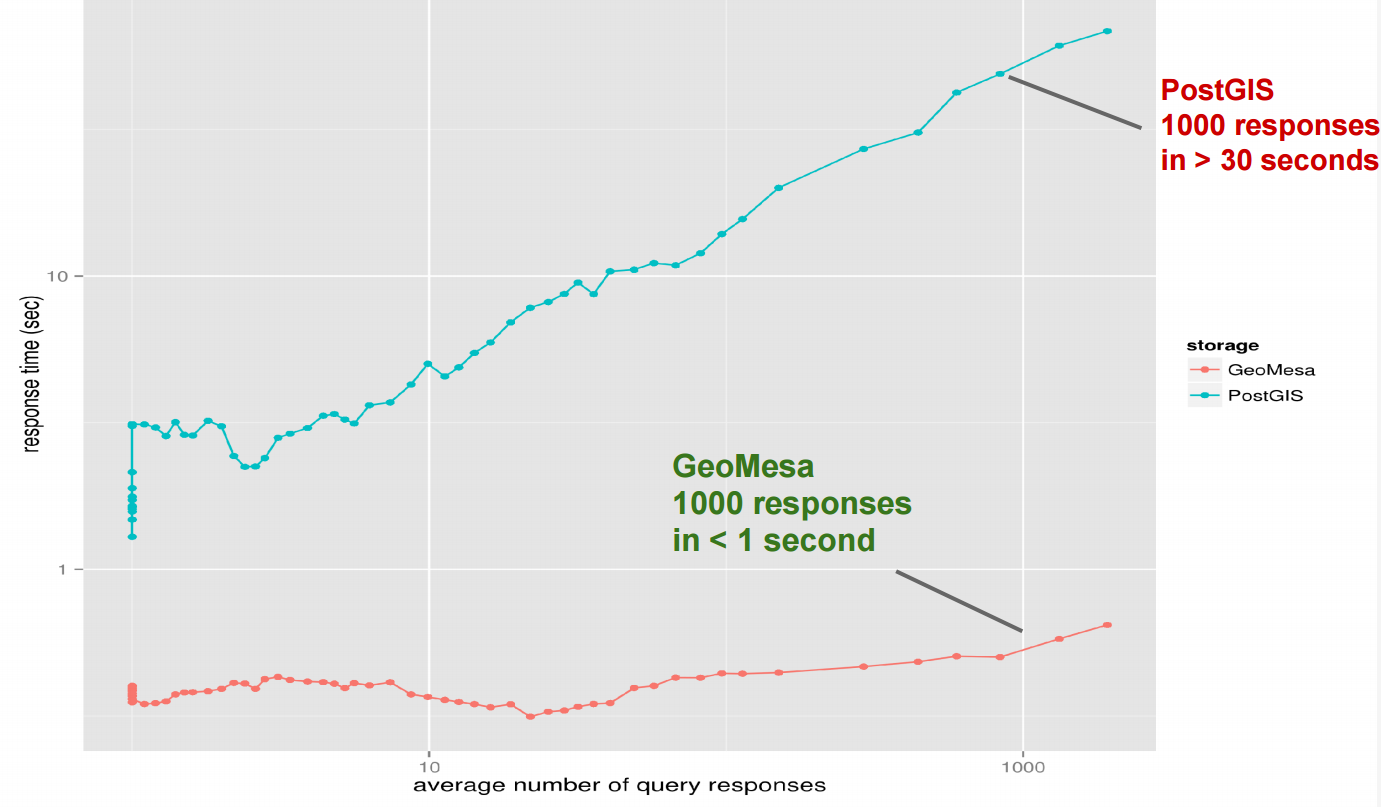
\includegraphics[width=.8\textwidth]{Abbildungen/geomesa_versus_postgis.png}
\caption[Antwortzeiten von GeoMesa und PostGIS]{Antwortzeiten von GeoMesa und PostGIS, Quelle \cite[S.24]{website:slideshare:geomesa}}
\label{fig:geomesaversuspostgis}
\end{figure}

Postgres-XL: Bis zu sechs fache Antwortdauer von PostgreSQL gegenüber Postgres-XL in einem standardisierten TPC-H\footnote{\url{http://www.tpc.org/tpch/}} Benchmark bei Verwendung von vier DataNodes. Abbildung \ref{fig:pgxcversuspgsql} zeigt das Diagramm mit dem genannten Wert. Die x-Achse ist nicht beschrieben, weswegen eine Einschätzung der Werte nicht möglich ist.
\begin{figure}[h!]
\centering
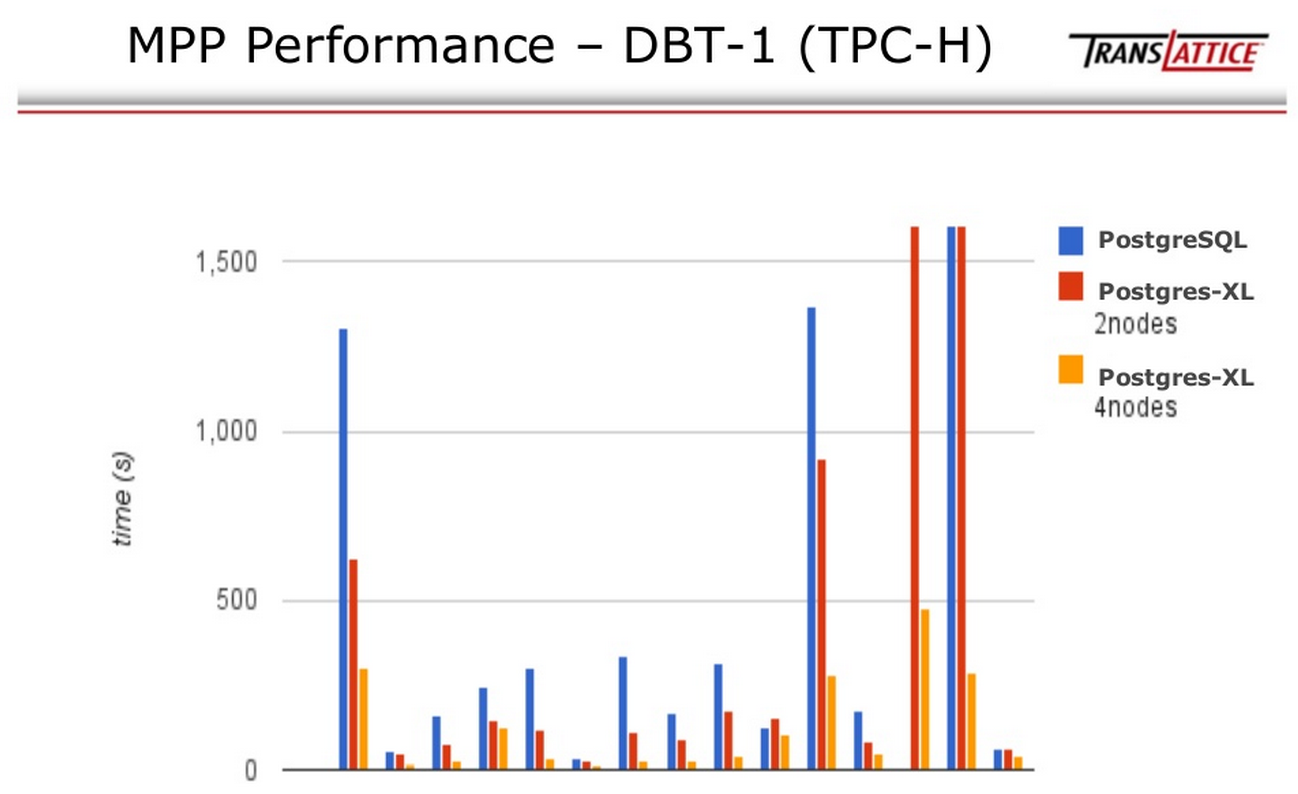
\includegraphics[width=.8\textwidth]{Abbildungen/postgresxl_versus_postgis.png}
\caption[TPC-H Benchmark von PostgreSQL und Postgres-XL]{TPC-H Benchmark von PostgreSQL und Postgres-XL, Quelle \cite[S.12]{website:slideshare:pgxc}}
\label{fig:pgxcversuspgsql}
\end{figure}

%nichts da, weswegen interesant zu erforschen